\chapter{Methodology}
\label{methodology}

\section{Project Management Methodology}
  \subsection{Workflow}
  The workflow one has designed has been inspired by existing 'agile' methods. It will consist of a single cyclical workflow, with two nested "sub workflows" whereby upon completion of a step, it is sometimes necessary to loop back on oneself to perform futher refinement; as illustrated by the diagram below.
  \begin{figure}
    \begin{center}
      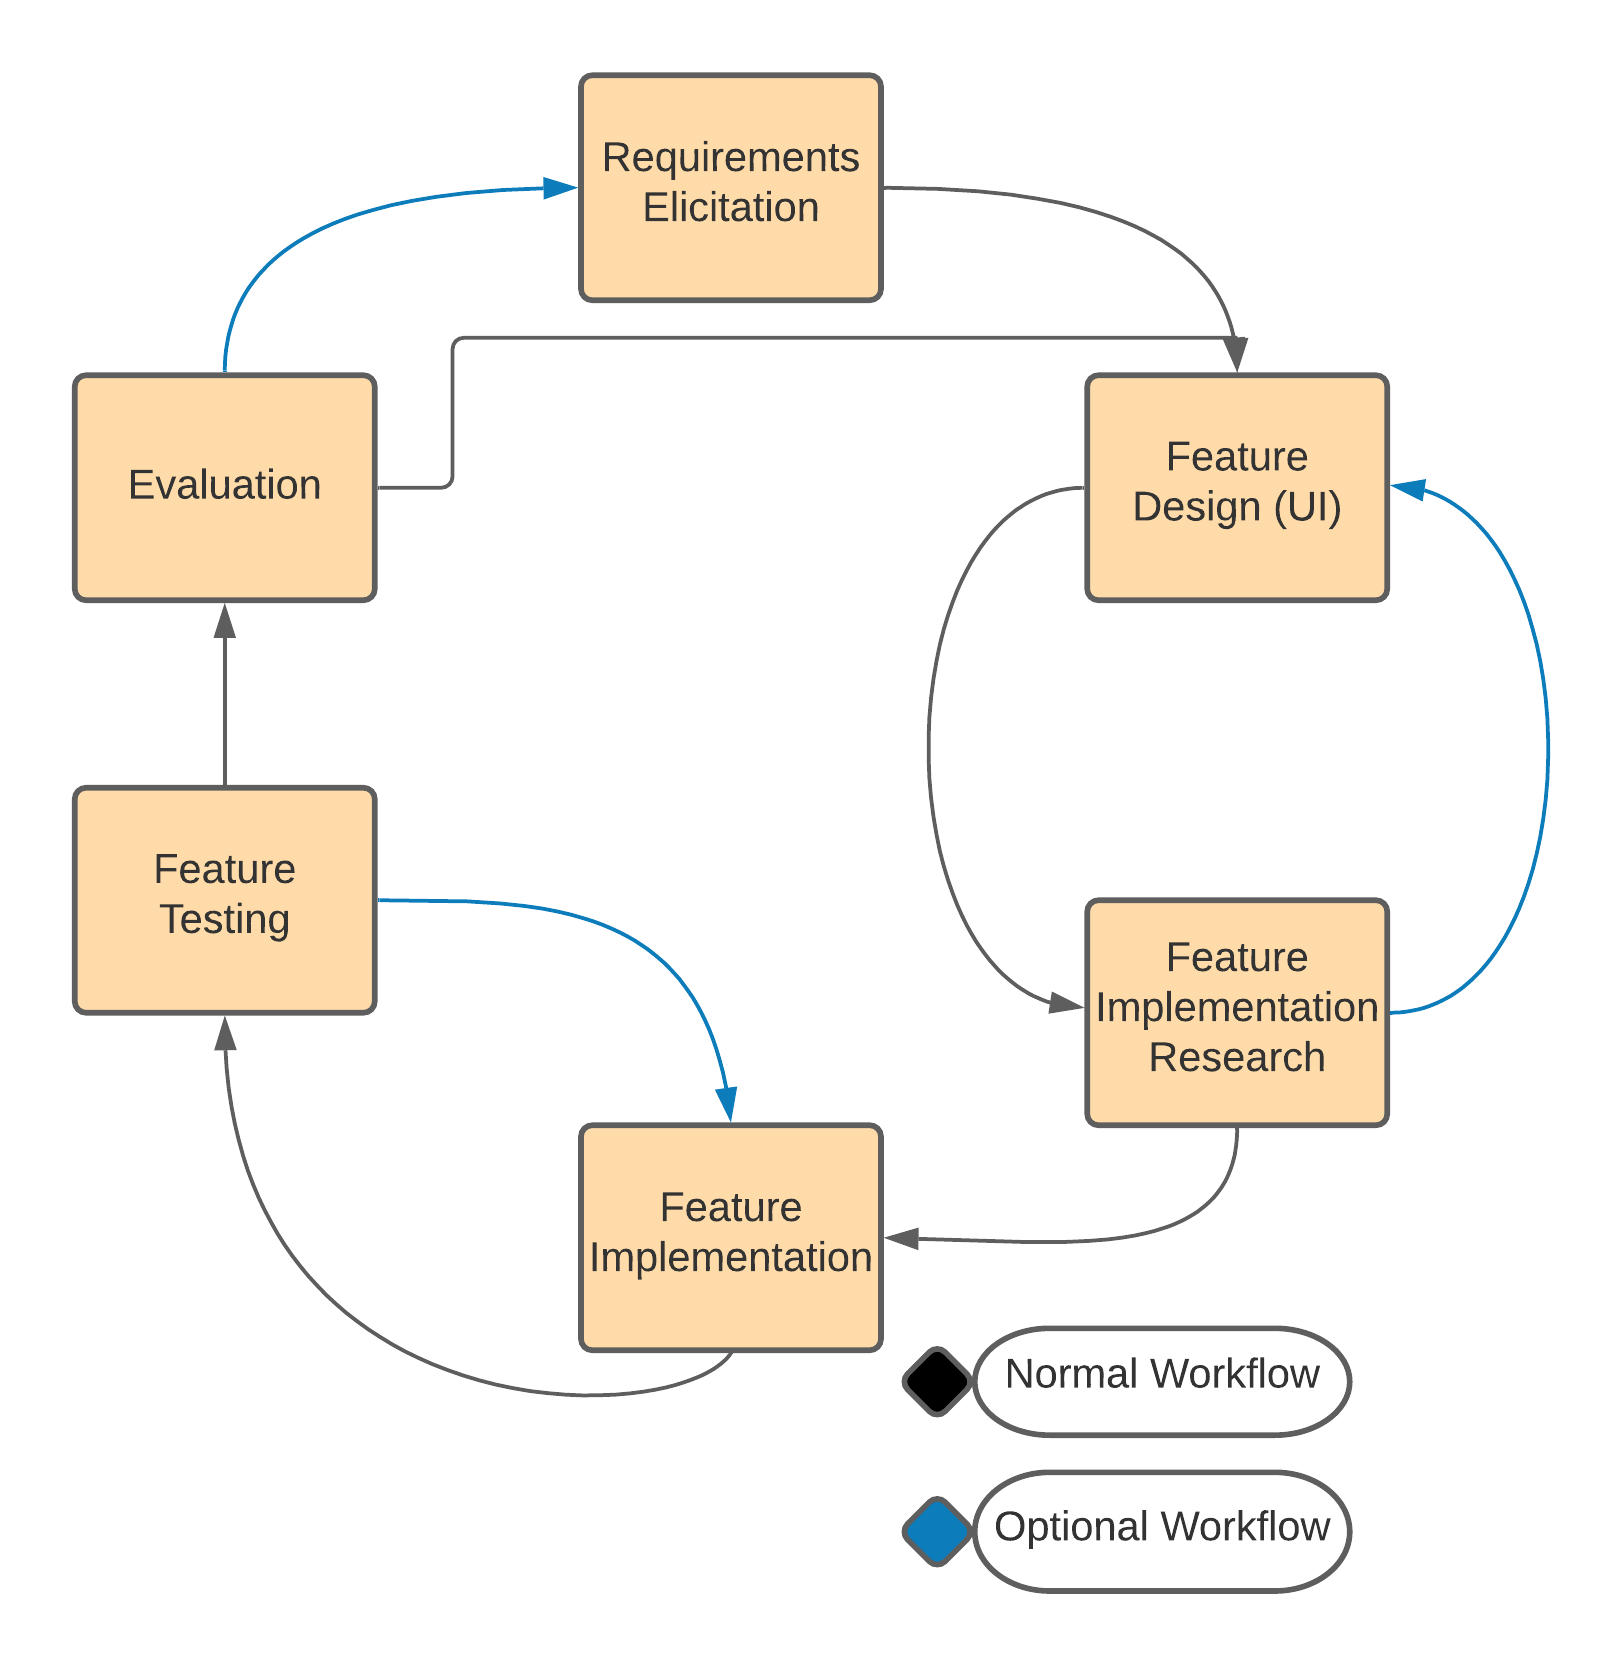
\includegraphics[scale=0.75]{Images/Project_Management_Methodology}
      \caption{Development Lifecycle}
      \label{fig:development lifecycle}
    \end{center}
  \end{figure}
  Throughout the project the focus of the workflow will shift as illustrated by the diagram below.

  \begin{figure}
    \begin{center}
      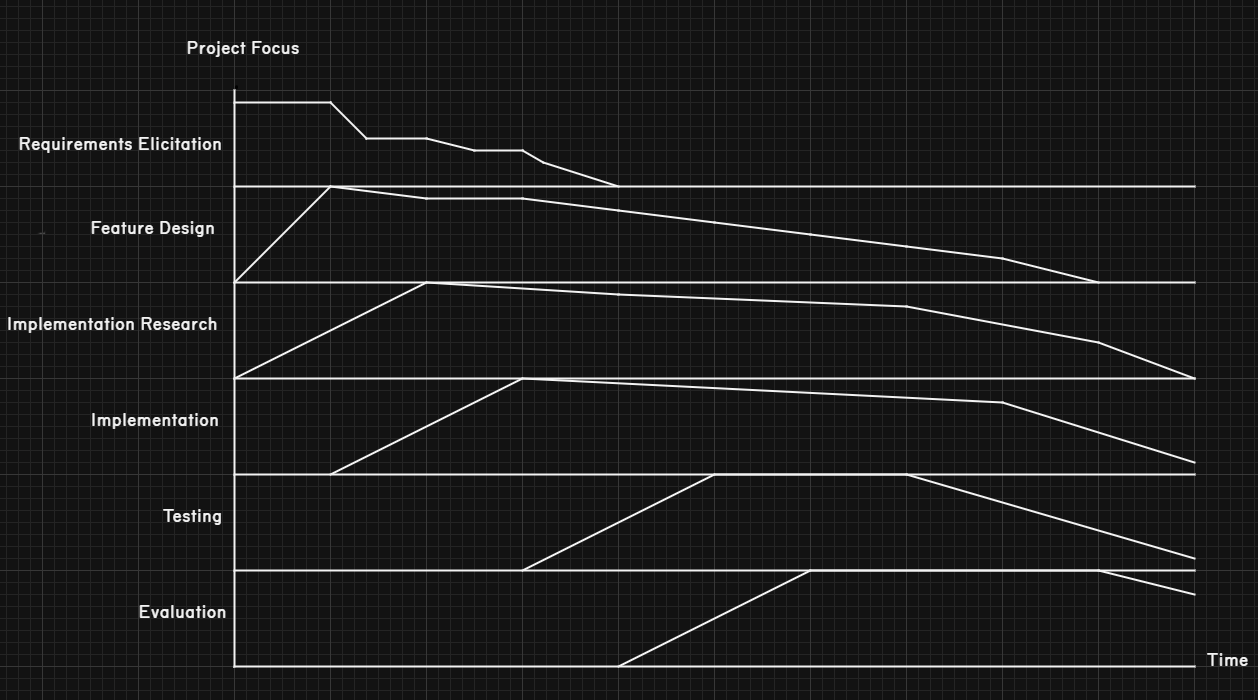
\includegraphics[scale=0.4]{Images/ProjectFocus2}
      \caption{Project Focus Over Time}
      \label{fig:project focus}
    \end{center}
  \end{figure}

  The paper \citep{Highsmith2001} makes a compelling argurment for the usage of 'agile' methodologies over more linear project management methodology (PMM) styles such as waterfall. 'agile' focuses on design being done 'on an ongoing bases in smaller chunks' \citep{Highsmith2001}. It is also highlighted that 'agile' allows development to respond to feedback and change. In fact 'agile' has customer, designer and developer feedback baked in to it's formula in the form of regular team meetings, especially if using the SCRUM 'flavour'.
  \par
  For a lone developer 'agile' with Kanban is the PMM of choice for this project as it allows the flexebility to iterate on designs as one learns more about the technologies being used and gives the freedom to modify one's requirments in light of newly found research and technical limitations. Aditionally, the nature of 'agile' is to have short lifecycles which has the virtue of frequent milestones. This allows one to better track progress of the project by being able to see how many tasks have been completed on the Kanban board during the development cycle\footnote[4]{Granted tasks alone are not the be-all, end-all metric but it does give some idea of progress}.
  \par
  Using Kanban to track tasks makes sense for a single developer as appose to using feature driven development. As this allows for non-programming tasks to be tracked in the same way as programming tasks.
  \par
  Furthermore, 'agile' is a worthwhile methodology to use and familiarise oneself with as it is becoming the new norm in industry; as shown by a study conducted by Hewlett Packard.

  \begin{figure}[H]
    \begin{center}
      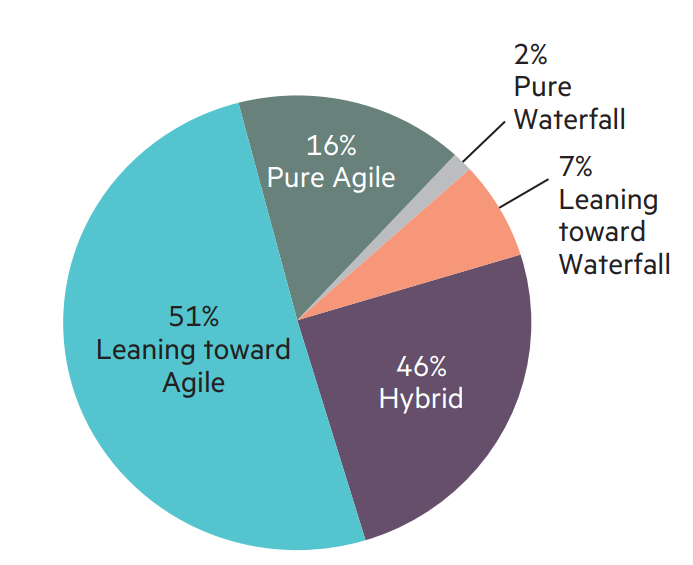
\includegraphics[scale=0.4]{Images/PMMPieChart}
      \caption{Primary development method used in organization across projects (601 respondents) diagram created by Hewlett Packard}
      \label{fig:PMM_PieChart}
    \end{center}
  \end{figure}

  \subsection{Requirements Elicitation}
    This involves determening the needs of the user and defining requirements to meet those needs.
    As the requirements will be determined by the developer in this case, reason being, the scope of the problem domain is narrow in terms of interaction points for the user. The following rationale will be used.
    One will create requirments that contribute towards providing information about crop defects to the user.
    Also, as the system is intented for use by non-technical persons, the interaction should be minimal, and clear. This means not cluttering the UI with too many points of interaction, making it clear what the application is doing at any given time. And using non-technical language, especially avoiding jargon.
    % As the scope of the problem domain is narrow in terms of interaction points for the user. Requirment elicitation will be driven by determining features that will build towards the solving the problem at hand. If for instance the problem was providing some kind of E-commerce website, project management application or social media website, the number of different features that could be employed in any one of these domains is vast and therefore one would need to consult the target audience and elicit the kind of requirements they would like to have. On the contrary, this project is far narrower in terms of points of interaction for the user. Therefore requirements will be determined on the basis of whether or not they contribute towards providing information about crop defects to the user.
  \subsection{Feature management}
    To track the creation and completion of features, a Kanban board will be used. This will include columns for 'To do', 'Doing' and 'Done'.
    To determine which features will be prioritised one will employ the MOSCOW method (See Requirements).


  \subsection{Evaluation Methods}
    This will be conducted by linking users to the website with a link to an online survey alongside a link to a google drive folder containing relevant test images. With the questionaire mostly consisting of System Usability Survey (SUS) questions. And some aditional bespoke questions regarding accuracy of prediction. User feedback aside from the data collected from the SUS survey will also be valuable for this project, it is a good way to be allerted to any usability issues; such as bugs, difficulty understanding how to use the application (what icons mean, order to carry out steps etc) and difficulty seeing UI elements due to poor colour choice.

\section{Development Methodology}
  \subsection{Feature Design}
    \subsubsection{UI}
      Wireframes will be uitilized to establish interface element placement i.e. layout. Then more mockups that align better with the possible implementation will be created superseding the original prototype wireframes. A colour picker that takes predetermined segments of the colour wheel, will be utilized to define the colour scheme. In later iterations of the design, once there is a functioning UI, usability will continue to be refined with the help of existing usability research, to guide the usage of font/colour/highlight on hover/font size etc. Additionally once a desktop friendly layout has been established, work will begin on optimizing a version for mobile.
    \subsubsection{Backend}
      To better conceptualize the needs of the user. Use case diagrams and activity diagrams will be utilized. Then the main types of code to help with design are psuedocode which is written loosley in a programming style but does not excecute. Prototype code, which runs but is intented to be discarded. And tracer code, this is a kind of MVP but on the individual feature level, which becomes the starting point for further development.
    \subsubsection{Design \& Implementation Coupling}
      An iterative aproach has been chosen because the design of the software is affected by factors of the implementation. Before implementing a feature it is not always clear how the solution will look and which possibilites will be simplest to meet the requirements. Therefore, an initial design will be created to guide the first steps of implementation, then as more information is learned and perhaps an easier to make design is realised, the new design can be checked against the requirments. If satisfactory, the new design can become canon and development on the updated design can continue.
      \par
      This coupling brings about the necessity of Won't have catagory in the MOSCOW method. This prevents future iterations of design and additional requirements encroaching on what the program will not be able to do. This can arise as an implementation choice may rule out the possibility of other features being included. For example the choice to use a sub-optimized javascript library may rule out the possibility of the application running on mobile.

  \subsection{Implementation}
    The first step will involve determining the apropriate technologies and libraries to achieve the design. This is necessary to realize the constraints that are imposed by the implementation method and know to what extent the design is feasible.
    \par
    The process to create the feature will then be carried out iteratively. When development begins we first arrive at a base-case often known as a Minimum Viable Product (MVP), often hard-coded solution and subsequently make the code more dynamic, flexible, and robust to erronus data. Then if necessary optimize the perfomance of the code to improve run-time. Ensuring to adhere to the software development practices outlined in the literature review.
    \par
    The ideal MVP will be one that fulfils the 'must have' requirements. Then it will be possible to expand it's features to include 'could have' features etc. Aditionally, once the MVP is acheived, design considerations such as ease of extensability and addition of new features will be more heavily focused on. Sometimes with major code refactor occuring at this point (see Refactoring), as to acheive the MVP quickly it is sometimes necessary to implement features in a way that may not be conducive to easy maintinence, efficency, readability or serving content dynamically. As noted in the literature review, this process of gradual addition of complexity is supported by many authors.

  \subsection{Testing methods}
    Testing will be conducted iterativley as the functionality expands, with unit tests being introduced for some components depending on time constraints. Testing will consist of firstly confirming that when interfaces are interogated with sound data, the responses are consistent with requirments. Secondly stress testing the interfaces with extraneous data will be carried out to ensure that apropriate error responses are given and the application does not simply crash. We ensure that if in the case of crashing, it is able to automatically re-start.
    \par
    On a larger project, especially if working with multiple developers, developing to test and having unit tests for each module is imperative. These test the module with valid and extraneous data against it's interface 'contract' i.e. what it promises to produce upon interaction. Secondly, integration tests would be created that test the interatction between modules. As integration is the most likely point for bugs to occur. When discovering a bug, it is good practice to create a test to reproduce it, firstly to cut down time checking if the bug is fixed, and to ensure it does not occur again.
    \par
    On a sufficiently large project it is also good practice to test the tests, by creating branches of the software that deliberatley fail, to ensure the tests are functioning correctly, and catching the errors you expect them to catch.

  % Throughout iterative process of creating the application, the design of the software is affected by factors which have a cause and effect relationship with one another. Following are some hypothetical scenarios that illustrate this point, such as; one decides to use a novel, bleeding edge, front-end javascript library to aid in creating user-interactive graphing of data. After creating a substantial poriton of the UI functionality, and finding it working smoothly on a high-end desktop PC, one decides to test the application on a smartphone, only to be left with the problem of extremely slow responsiveness. One is then left with the realization, that the novel UI-library is far from optimized and one is now forced in to a bind. If requirments don't specifically request mobile functionality then it would be possible to carry on using the library, however, if one is to take this route, one should have stated in the requirments 'Won't have mobile device support'. However if requirments dictate that mobile support is a 'Must Have' or even 'Should-Have' two main possibilites arise, either the library is being used inefectually and time is needed for the developer to become proficcient at using it. Or the library is simply slow. If for whatever reason the library must be dropped from the project, aspects of the UI design will need to change, to better reflect the reduction in expected features; this being caused by the extra time taken to implement what was previously offered by the library. Either this, or extending the project deadline. A final example is a situation whereby an application stores and handles sensitive information about a user, for instance an online medical checkup. This can lead to large poritons of a codebase needing to be re-factored and documentation updated, if later in the development process the team discovers a security vunerability in a technology or library they are using. Modifications may involve updating class diagrams and system overview diagrams etc.

   \subsection{Refactoring}
   an example to illustrate the process of refactoring that will be utilized during development. The first peice code was arrived at because the base case was to retrieve the most likely defect. The extended requirment was to find the top three most likely defects. This has resulted in two methods being created for each case as the base case was coded first and extended requirment added in later. Although this is still functional, it's unnecessary and the code can be simplified, by using the result produced by the newly created method, the base-case method and any calls to it can be deleted. (note the method is declared in Model class which has been ommitted for clarity) Refactor example one, three, is entirely debateable as to whether or not it is an improvement. It is certainly more terse, which makes it arguably more difficult to read. The counterpoint to this being,  one is not allocating a computationally redundant variable at runtime. This being moreso noteable in the language of Python. Given it's interpreted nature, the interpreter will garunteed cause the machine to execute this operation (granted it's a fairly inexpensive one). If it were a compiled however, it is likely the compiler would ignore this redundancy and it would have no bearing on the speed of the program. Finally, comments are either added or updated.

   \begin{figure}[H]
     \begin{center}
       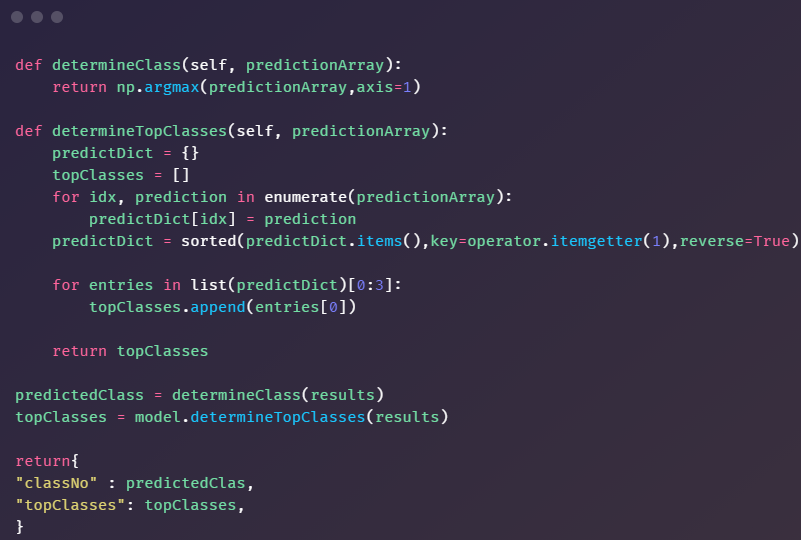
\includegraphics[scale=0.55]{Images/Refactor/refactorA1}
       \caption{Example 1 : Initial}
       \label{fig:refactorA1}
     \end{center}
   \end{figure}

   \begin{figure}[H]
     \begin{center}
       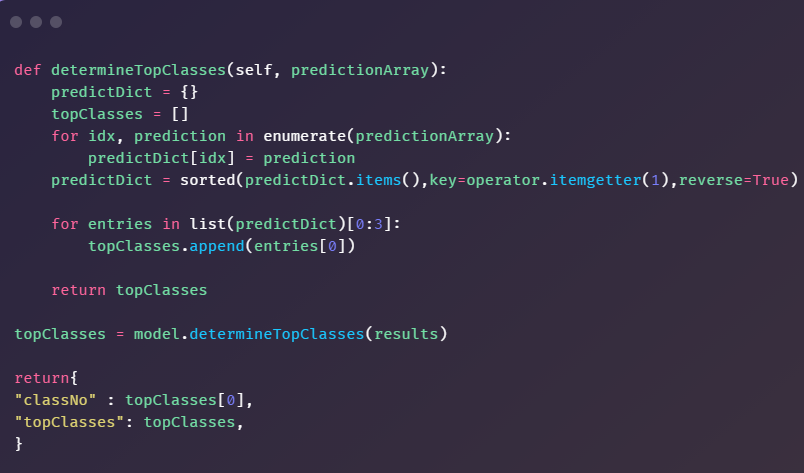
\includegraphics[scale=0.55]{Images/Refactor/refactorA2}
       \caption{Example 1 : Refactor 1}
       \label{fig:refactorA2}
     \end{center}
   \end{figure}

   \begin{figure}[H]
     \begin{center}
       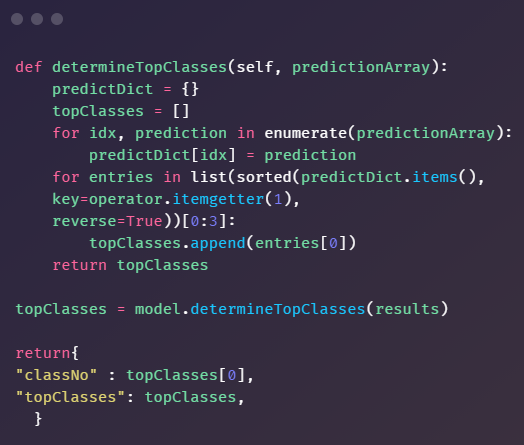
\includegraphics[scale=0.55]{Images/Refactor/refactorA3}
       \caption{Example 1 : Refactor 3}
       \label{fig:refactorA3}
     \end{center}
   \end{figure}

   \begin{figure}[H]
     \begin{center}
       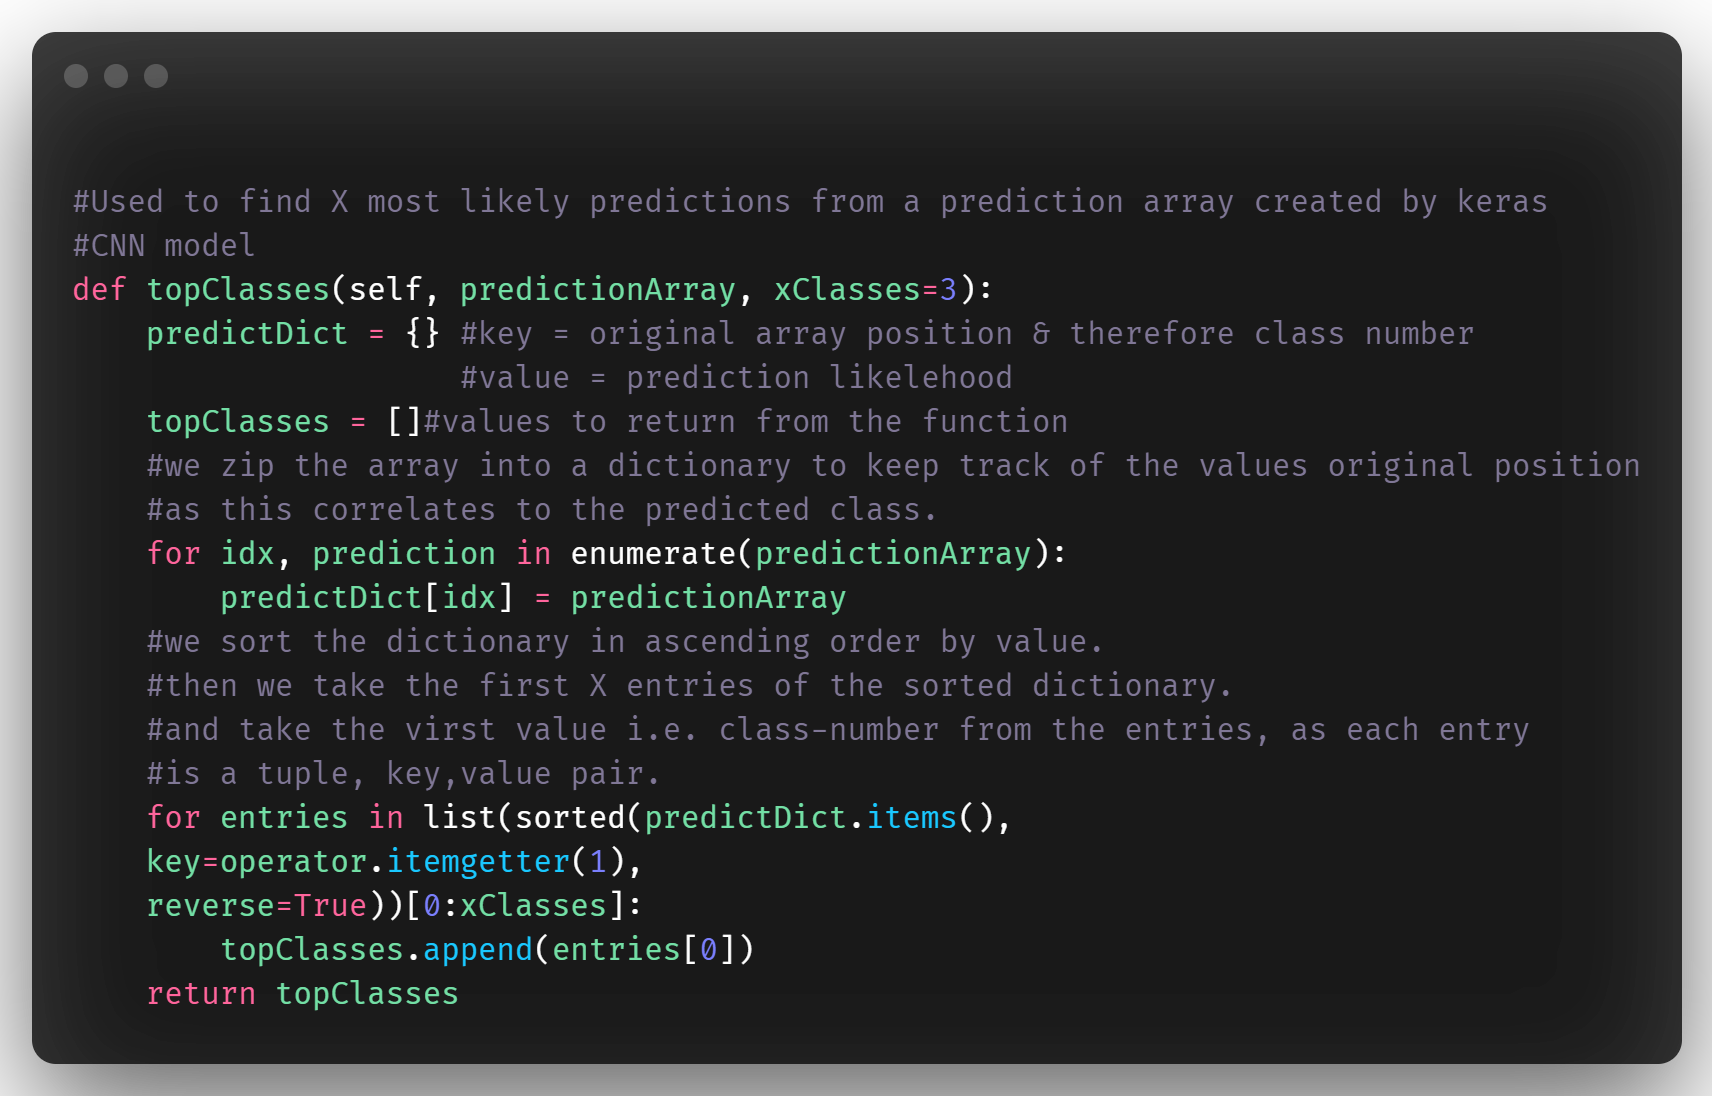
\includegraphics[scale=0.55]{Images/Refactor/refactorA4}
       \caption{Example 1 : Refactor 4}
       \label{fig:refactorA4}
     \end{center}
   \end{figure}

   In this example of refactoring we see how multiple redundant variable allocations can be condensed into a single line.
   \begin{figure}[H]
     \begin{center}
       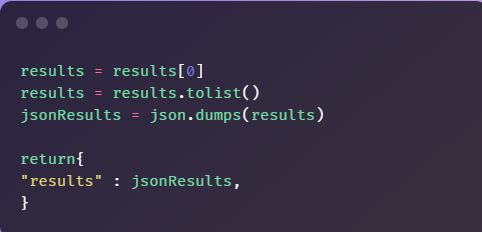
\includegraphics[scale=0.55]{Images/Refactor/refactorB1}
       \caption{Example 2 : Initial}
       \label{fig:refactorB1}
     \end{center}
   \end{figure}

   \begin{figure}[H]
     \begin{center}
       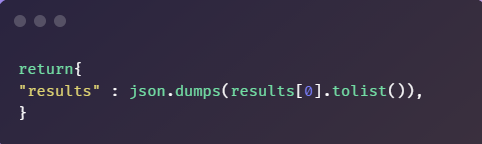
\includegraphics[scale=0.55]{Images/Refactor/refactorB2}
       \caption{Example 2 : Refactor}
       \label{fig:refactorB2}
     \end{center}
   \end{figure}

   Given these examples it's easy to see why lines of code created is a rather ineffective way (in isolation) of determening programmer productivity.

 \subsection{CNN Model Creation \& Integration}
  To create the CNN it is possible to perform modifications to an 'off the shelf' model included in the Keras library. The modifications involve changing the first and last layers to match the input image size and number of output classes respectively, we see this aproach used in several of the papers cited in the literature review.
  \par
  A fast to train model will be essential due to the limitations of using Google Colab, which requires frequent user interaction to prevent from stopping compuation or entirely disconnecting the run-time. Therefore a model with low-number of parameters will be chosen.
  \par
  The weights of the CNN will need to be saved after each epoch to ensure that if a disconnect occurs, less training progress will be lost. Once the model is finished training it will have it's class list extracted and the model weights will be saved into a .h5 file to be loaded on the API. The JSON class list will also be added to the API.
  \par
  When training the CNN one will utilize a pre-trained (on the ILSVRC dataset) to further cut down training time, as this will mean the CNN already has a set of generic feature maps. The focus on reducing training time is based on the fact that training large networks with millions of parameters can take days or weeks, even when utilizing high end GPU's.
  \par
  For the tradeoff in training time it is unlikely the model will acheive state of the art performance, but it is likely to achieve within a few percent. This has driven the requriement that the model must be easily replaced.

  \subsection{Version control}
    I will be using Git and Github. This will allow the creation of branches to explore experimental parts of the soloution space without disrupting the progress of the main branch. If the experimental implementation is successfull it will be merged with the main branch. It also allows the development of features in paralel, with any conflicts in their implementation being resolved at the merge stage. The inclusion of a remote repository allows for work to continue on a seperate machine if necessary and later be synced with the local main branch.
    \begin{figure}[H]
      \begin{center}
        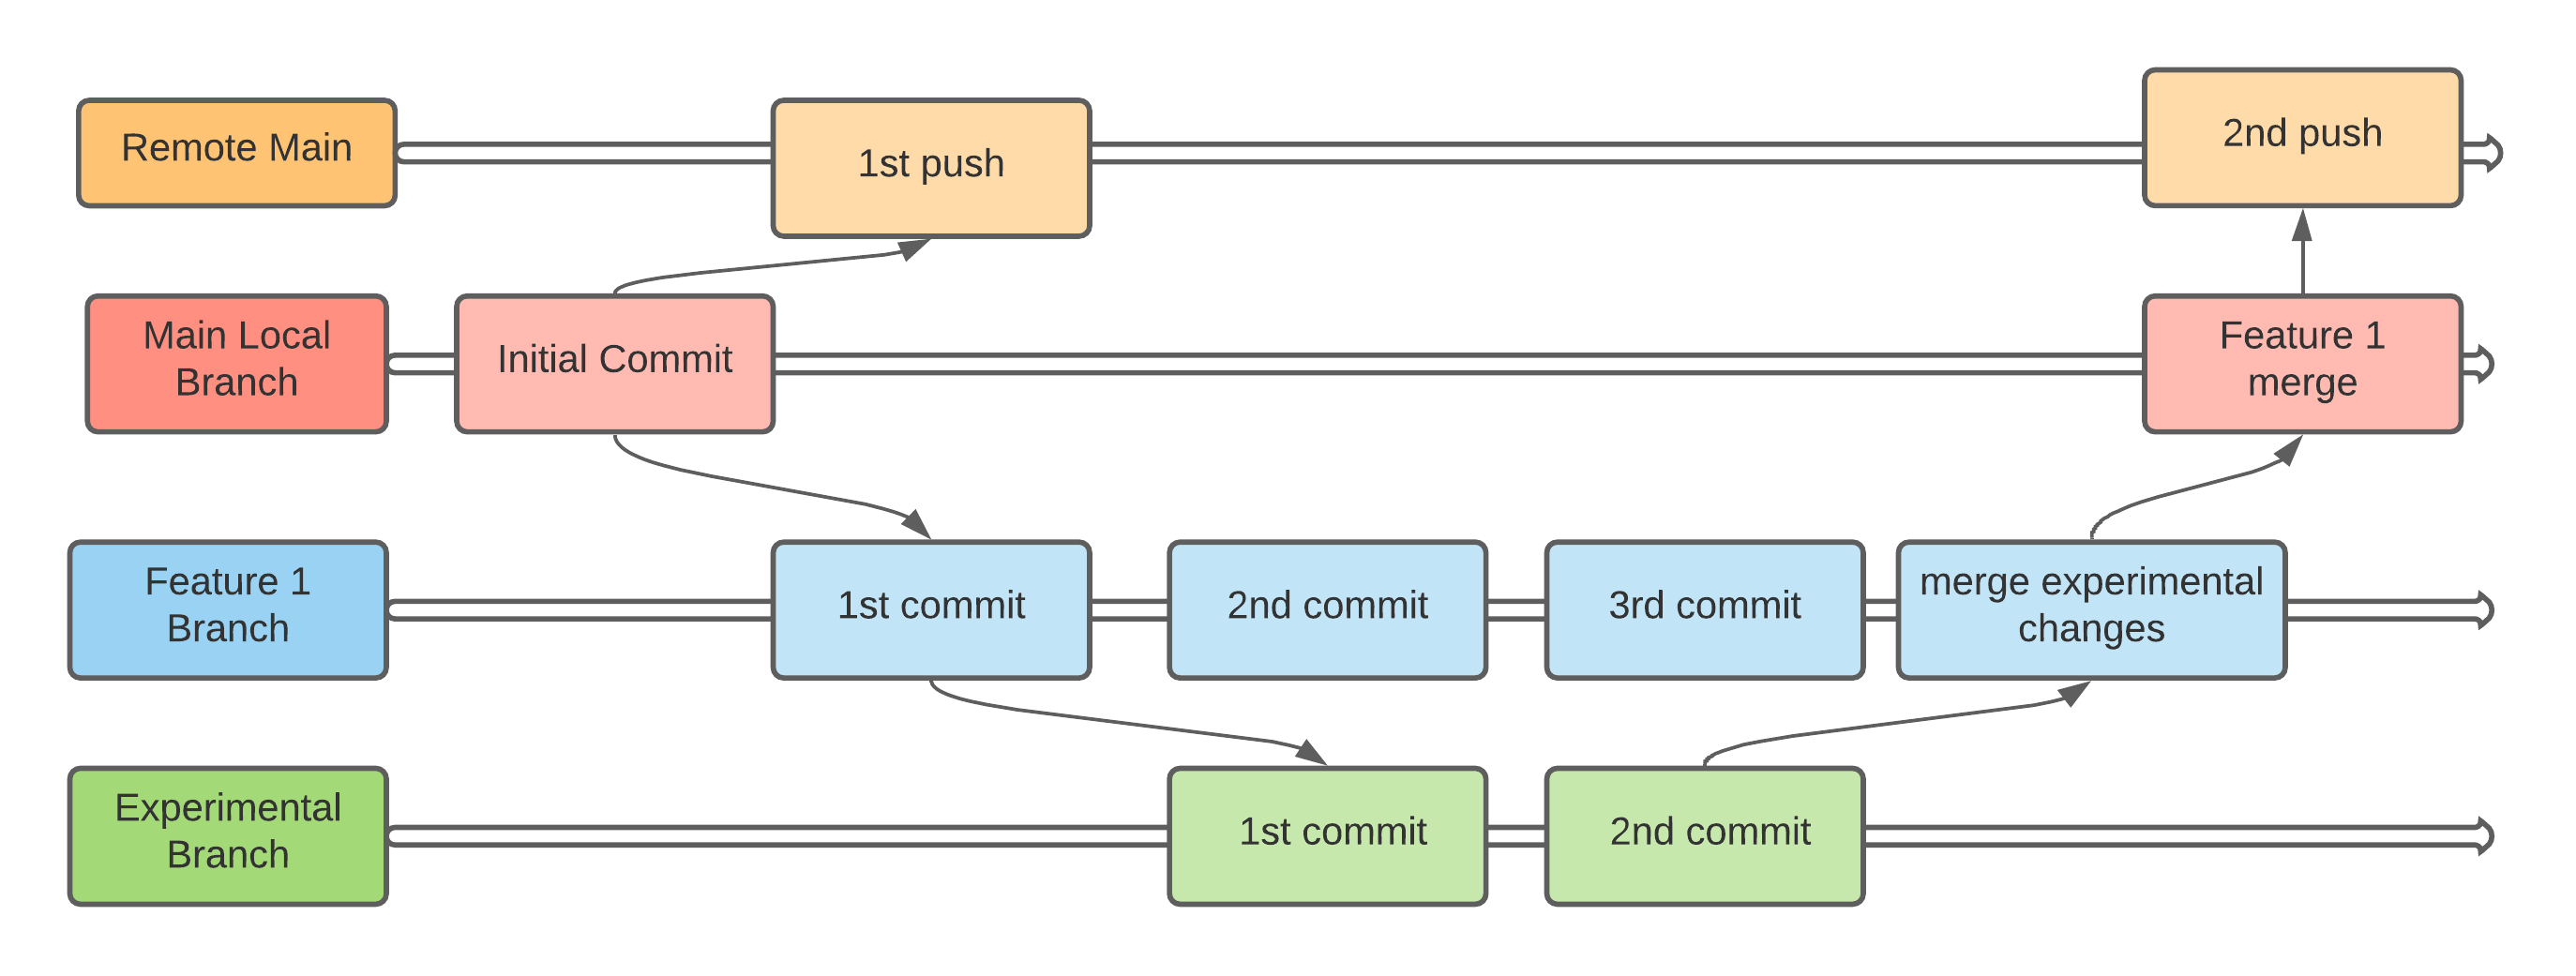
\includegraphics[scale=0.7]{Images/Git_Workflow_Diagram}
        \caption{Example Workflow To Highlight Branch Usage}
        \label{fig:Git Workflow}
      \end{center}
    \end{figure}

\section{Evaluation methods}
  \subsection{User Interface}
  The main method that will be utilized to determine the quality of the user interface will be the System Usability Scale (SUS) which can be seen here. (CITATION) % insert reference here
  The evaluator will be given remote access to the webservice. They will also be provided with some sample images to test the perfomance of the CNN incase they do not have suitable images of their own.
  The opinion data will be collected via online questionare.
  \subsection{Convolutional Neural Network (CNN)}
  Metrics for the evaluation of the CNN will be:
  \begin{itemize}
    \item Time to train the network on available hardware
    \begin{itemize}
      \item The constraint here being if the network cannot be trained on the available hardware in under sixteen hours. Purely for practical considerations.
    \end{itemize}
    \item Accuracy of CNN predictions. (which will be most effective when there are equal numbers of samples belonging to each class) $Accuracy = \frac{Correct Predicitons}{Total Predictions}$ else if the samples are skewed, the network could be a faliure at detecting a specific under-represented class, yet still score high accuracy.
    \item Precision. This is the number of correctly predicted images out of all predictions of that class. $Precision = \frac{Correctly Predicted for Class}{Total Predicted for Class}$ The network is precise for a class when the predictions it does make for the measured class are correct. Precicion cannot be used in isolation due to the fact that the network can have a high prediction for a class but still fail to identify the majority of images for that class. Succeeding soley on the fact that the images it has classified as the class being measured are correct.
    \item Recall. Is the correct number of predictions for a class out of the number present of that class. $Recall = \frac{Correct Predicted for Class}{No. Present For Class}$
    This metric can also not be used in isolation due to the fact it does not take in to account the number of false positives. i.e. The number of images incorectly classified as the class in question. For example, if an image dataset contained three classes A, B, C, and the classfiier labeled all images A. The recall for A would be 100 percent.
    \item F1 score. This metric tries to find the balance between precision and recall and can be expressed as $F1 = 2 \times \frac{1}{\frac{1}{precicion} + \frac{1}{recall}}$
  \end{itemize}
\section{Initial Designs}
Firstly I have created a wireframe UI
  \begin{figure}[H]
    \begin{center}
      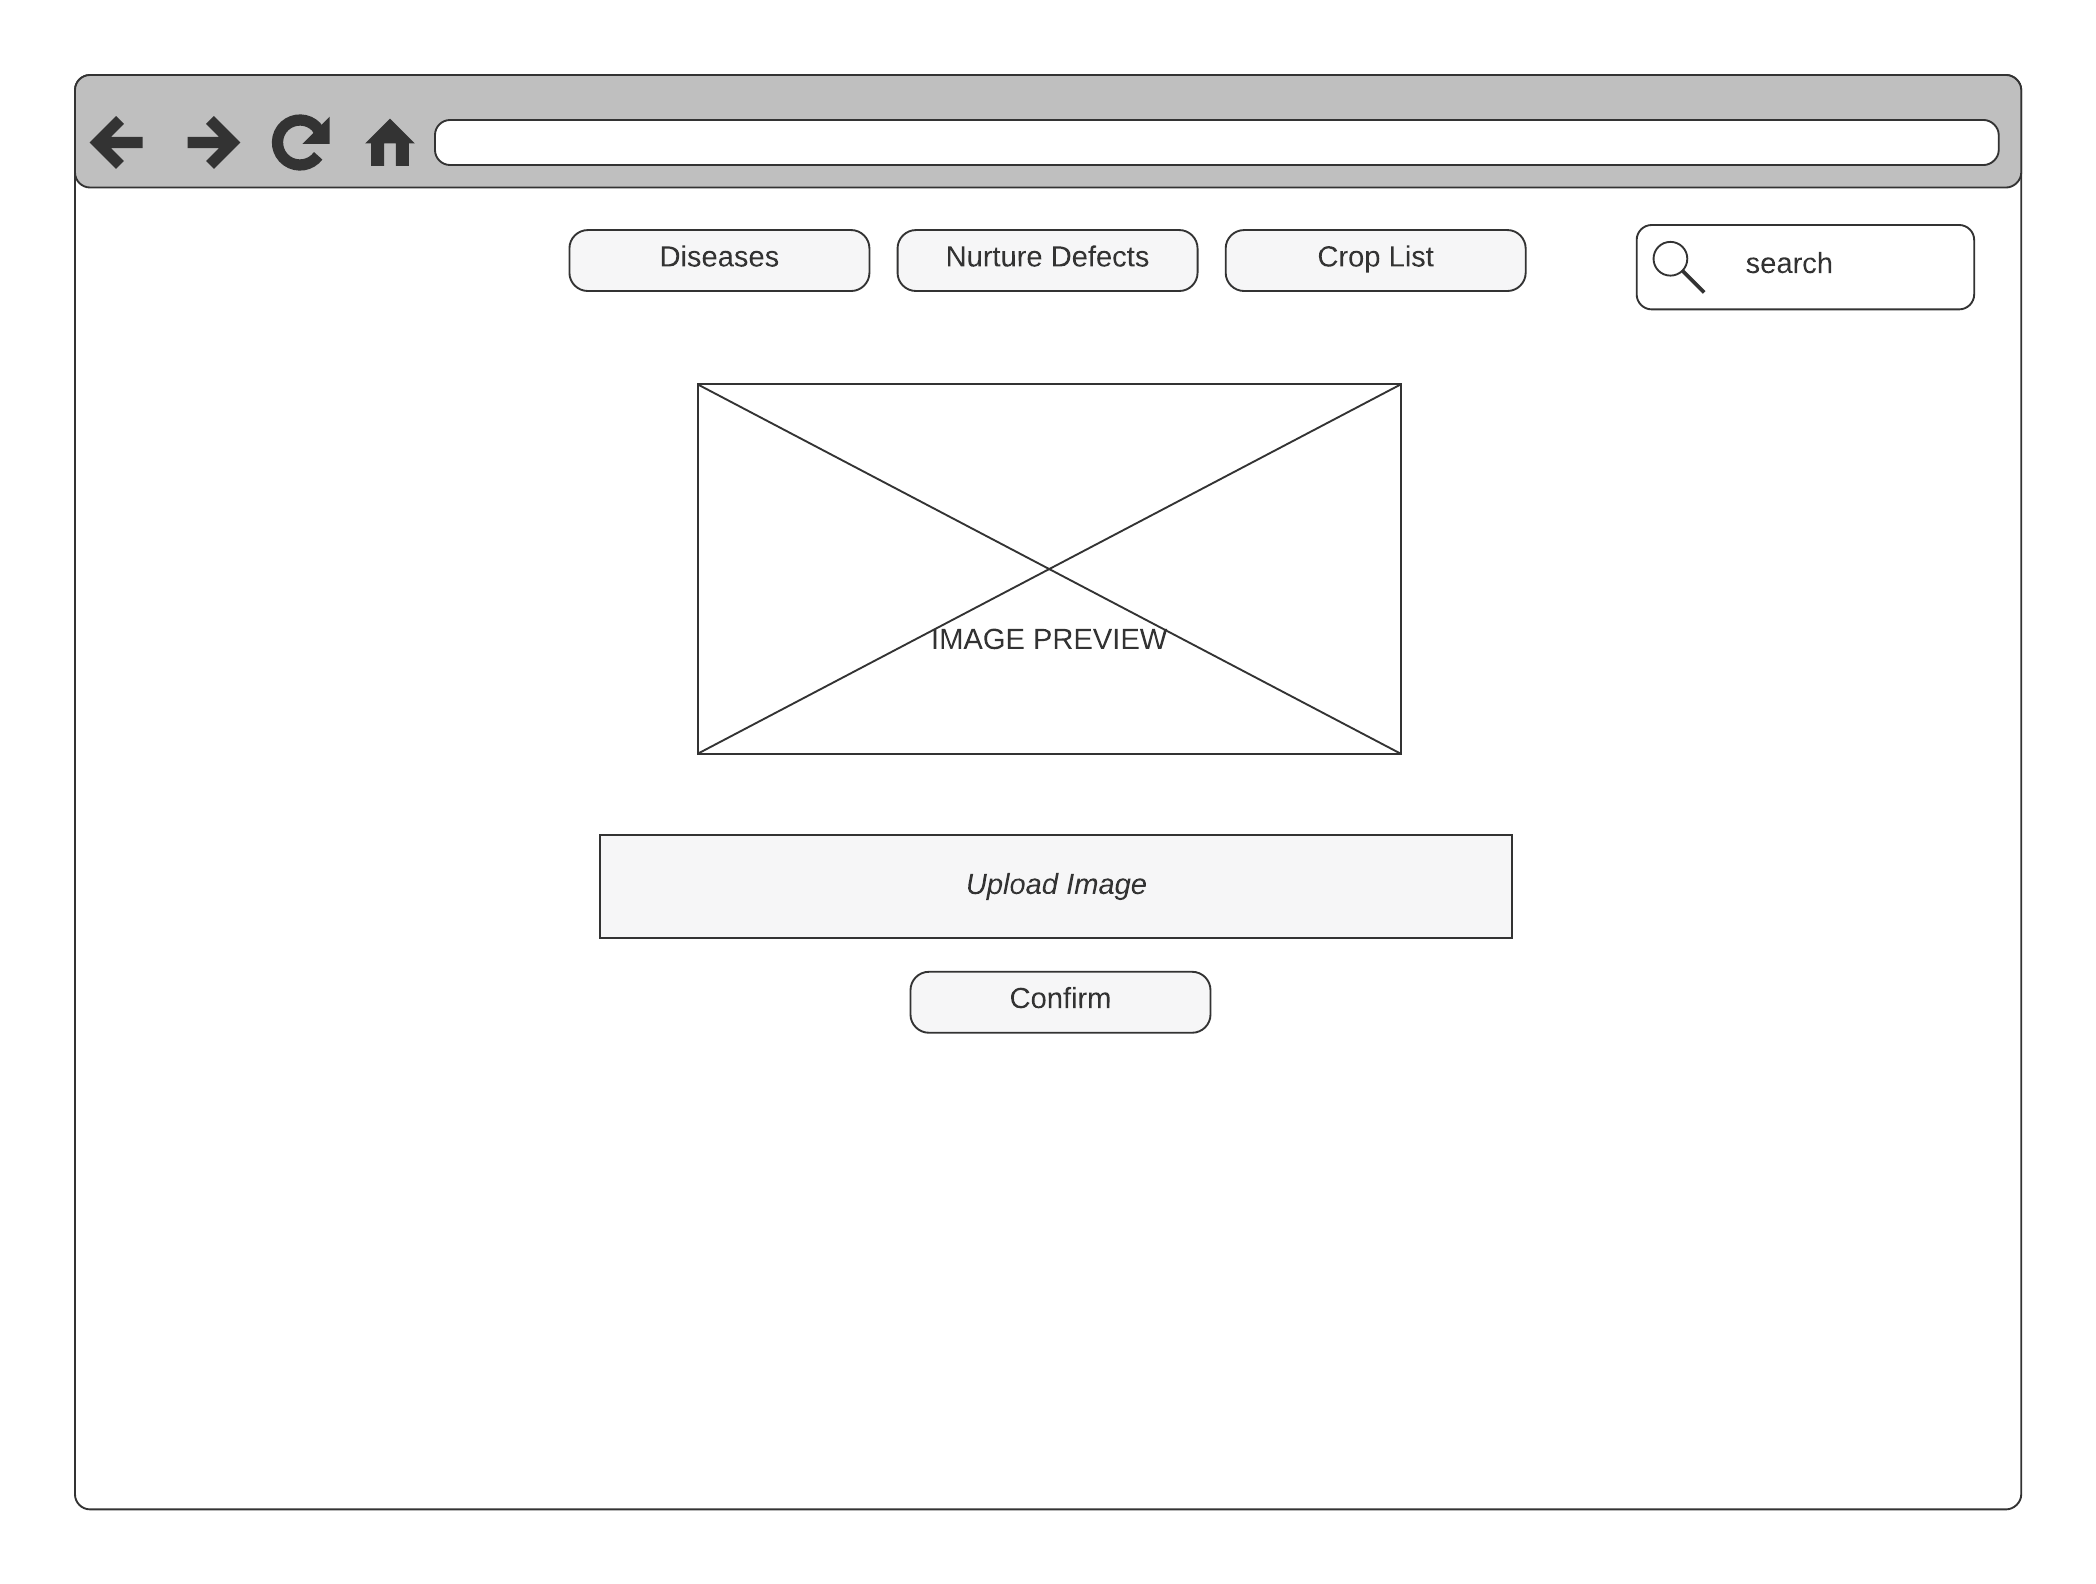
\includegraphics[scale=0.7]{Images/Home_Page_Wireframe}
      \caption{Homepage Wireframe}
      \label{fig:homepage_wireframe}
    \end{center}
  \end{figure}
  \begin{figure}[H]
    \begin{center}
      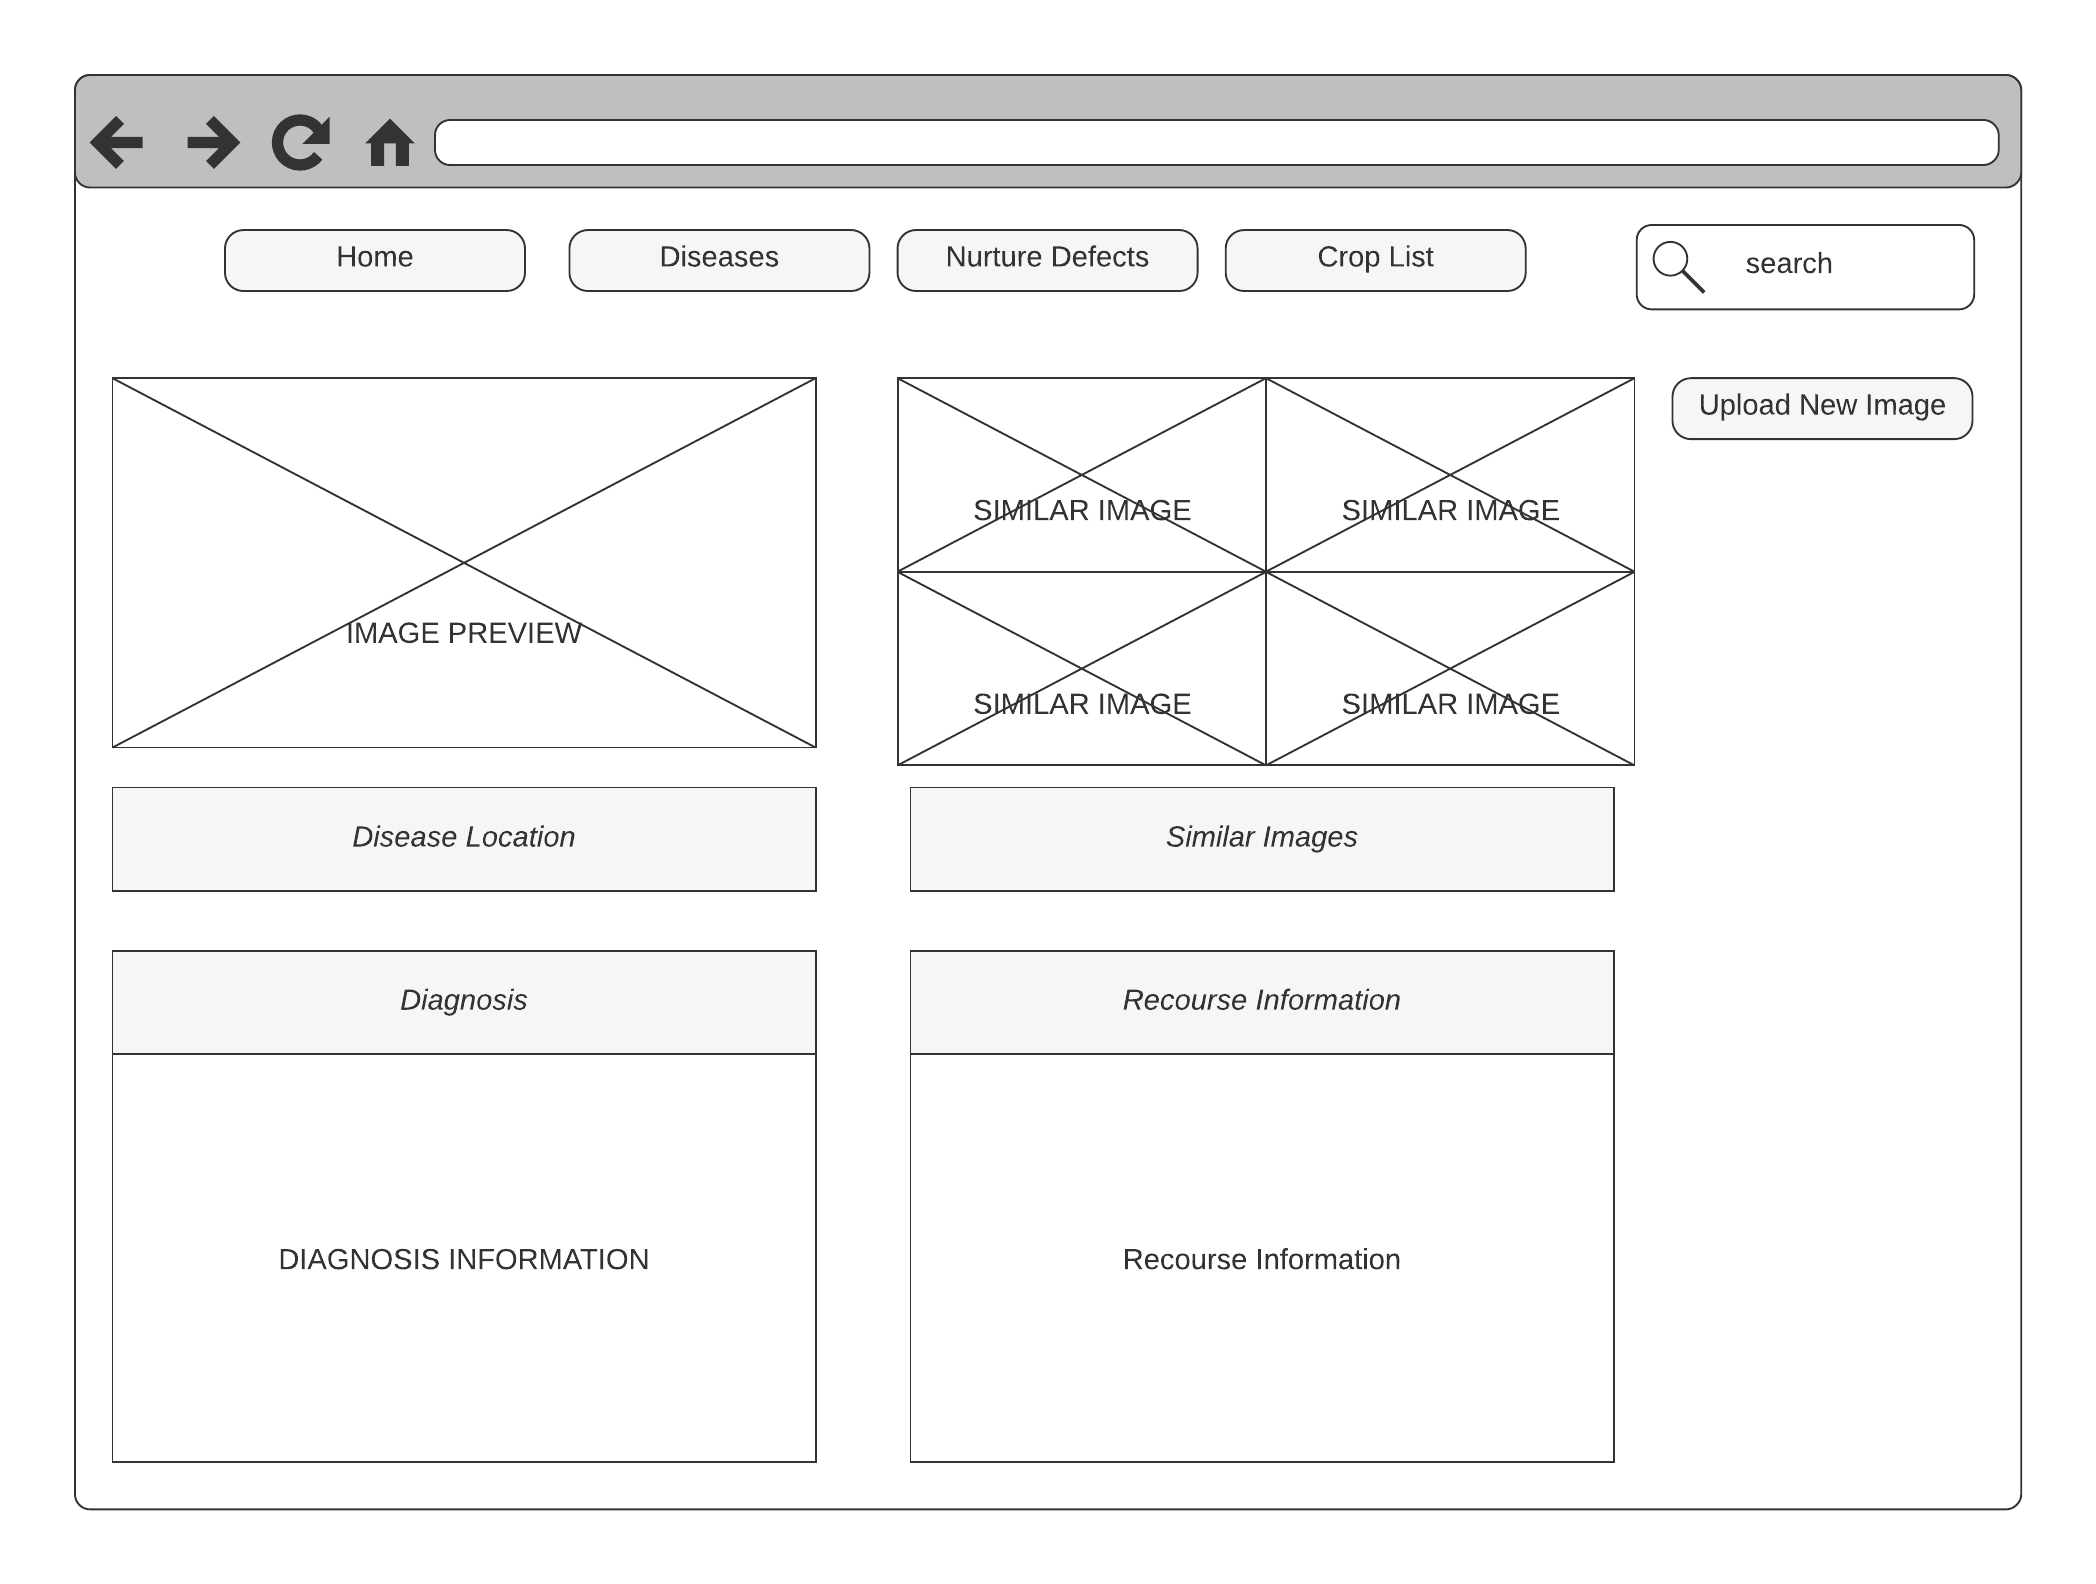
\includegraphics[scale=0.7]{Images/Defect_Information_Wireframe}
      \caption{Defect Information Wireframe}
      \label{fig:defect_wireframe}
    \end{center}
  \end{figure}
  \begin{figure}[H]
    \begin{center}
      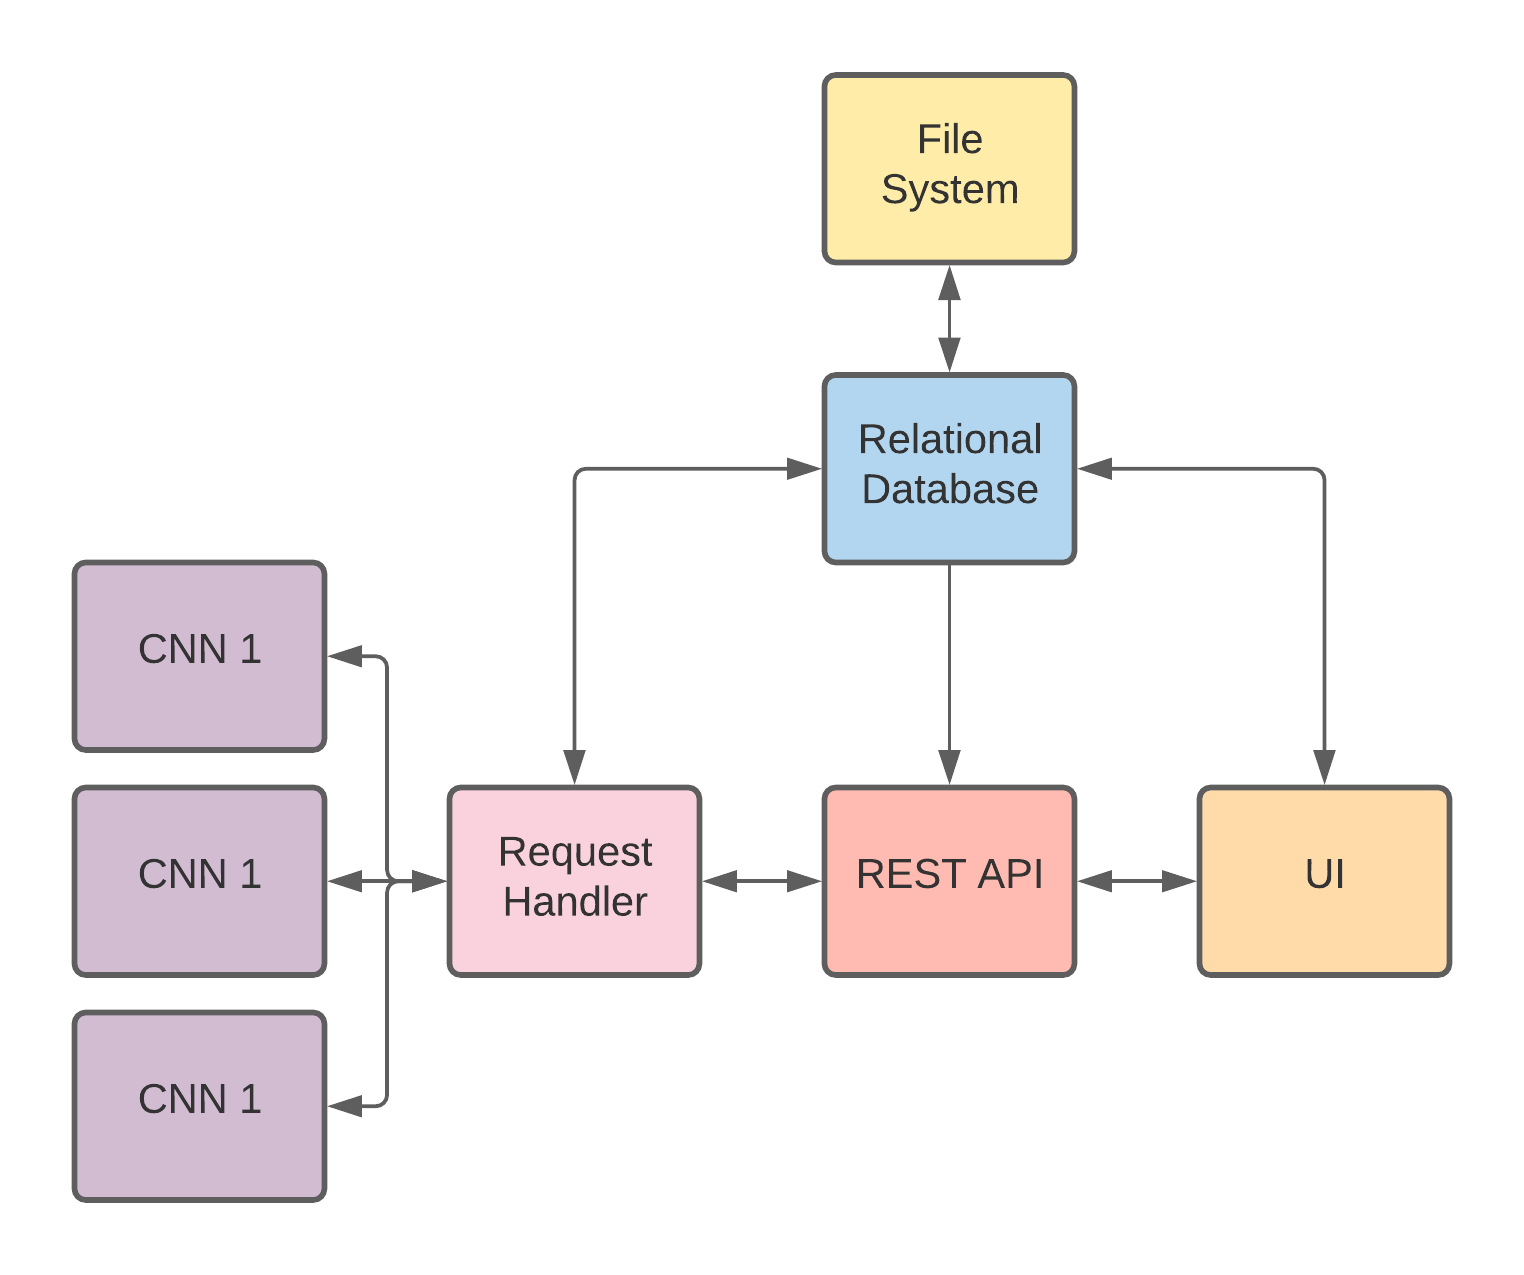
\includegraphics[scale=0.7]{Images/System_Overview_v1}
      \caption{System Overview}
      \label{fig:sys_overview}
    \end{center}
  \end{figure}
    \begin{figure}[H]
      \begin{center}
        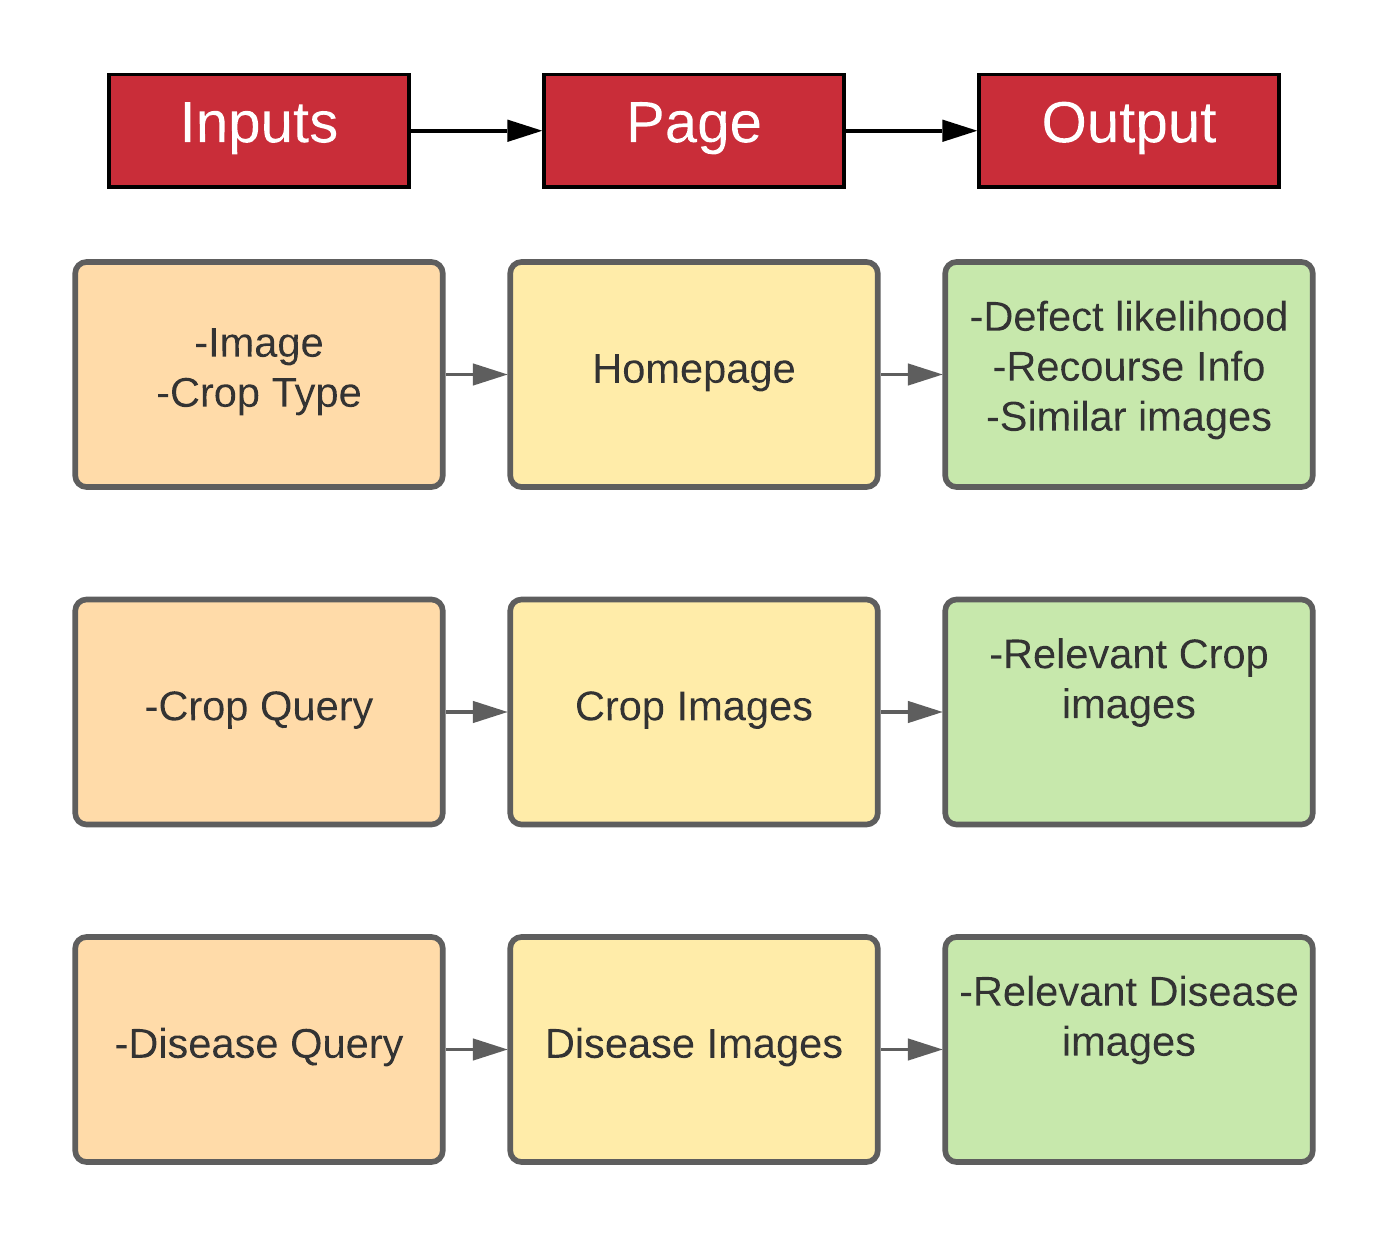
\includegraphics[scale=0.7]{Images/Input_Output_UI}
        \caption{Input/Output overview}
        \label{fig:input_output}
      \end{center}
    \end{figure}
    \begin{figure}[H]
      \begin{center}
        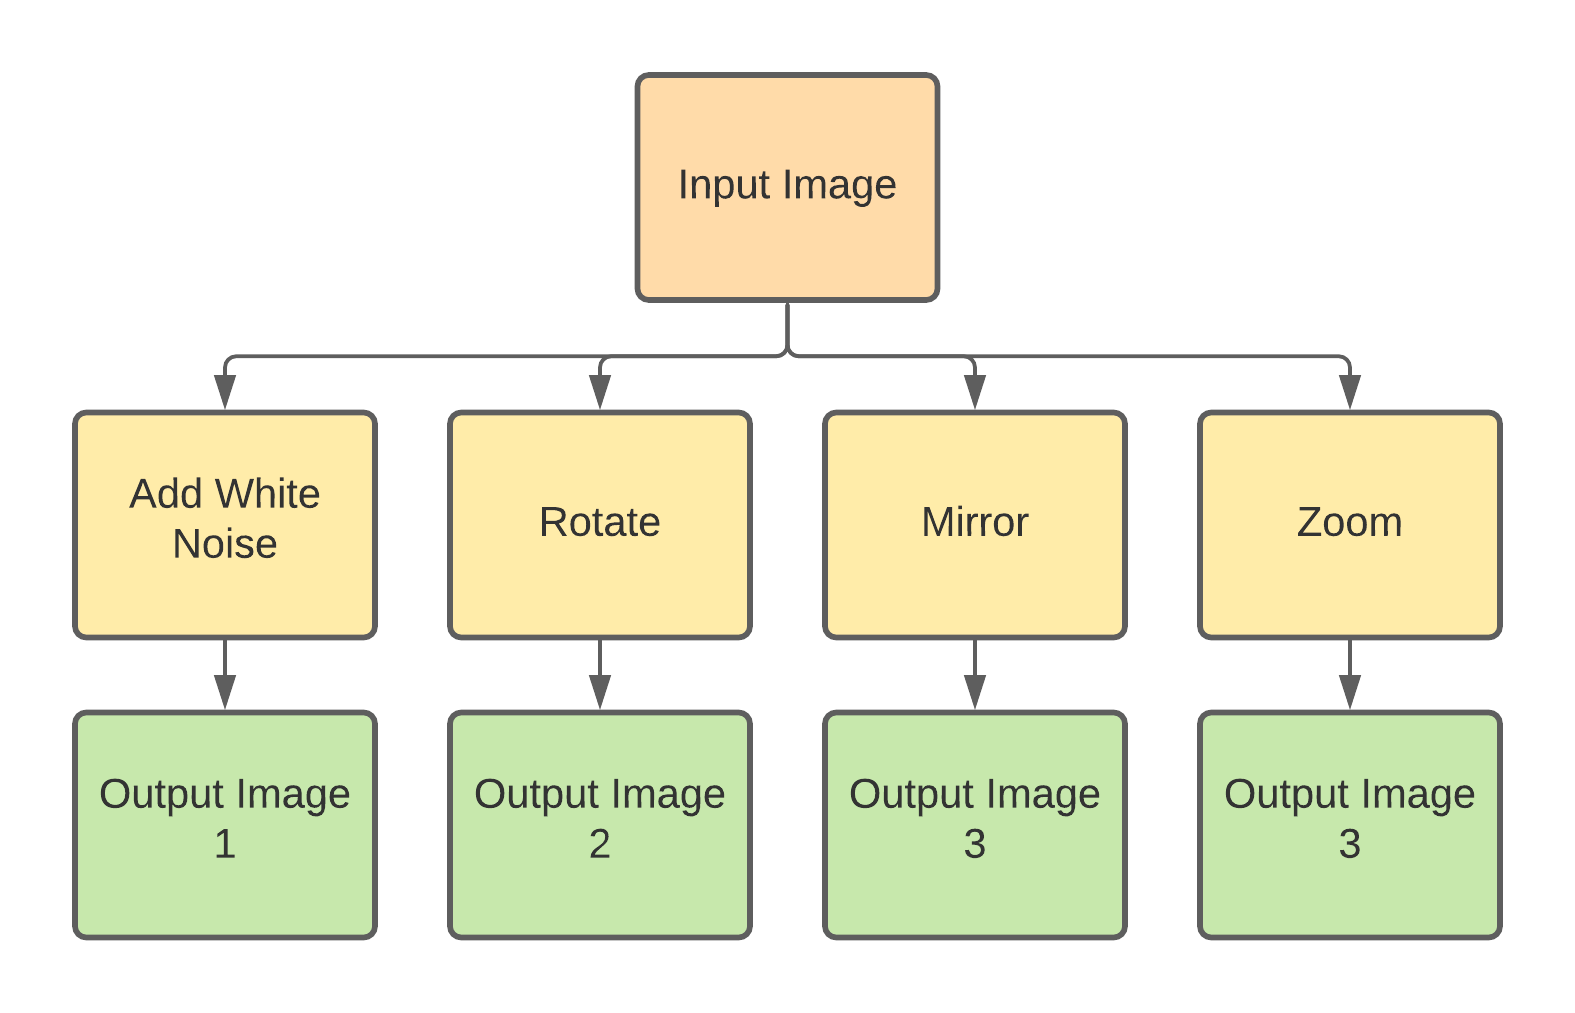
\includegraphics[scale=0.7]{Images/Data_Augmentation}
        \caption{Input/Data Augmentation Methods}
        \label{fig:data_augmentation}
      \end{center}
    \end{figure}
  See diagrams Apendix for additional diagrams.
\section{Employed Technologies \& Justifications}
  \subsection{Software Structure}
    \subsubsection{Back-End}
      The design aims to seprate the functionality of the CNN and the User Interface (UI) through use of a Representational State Transfer (RESTFul) Aplication Interface (API). The central idea of this aproach is to allow a seperation of distinct components which allows for flexebility in managing updates and changes to each component. The 'backend', which in this context, refers to the CNN and it's related functionality such as processing it's input's and outputs; will both receive input and serve it's output through the interface of the RESTFul API. each 'endpoint' or in other words internal class of the API will all inherit from the Resource interface which means it will recieve the main four HTTP protocol functions. POST, GET, PUT, DELETE. All interogations of the CNN will be conducted through these requests.
      \par
      A key feature of A RESTFul interface is the fact that no client information is stored
      between requests, this aids in making the interface more scalable and iteroperable. That is, scalable in the sense that increasing clients does not increase the amount of information the backend will have to store and be interoperable in the sense that any client, be it mobile appliation, CLI program or webpage can use the interface.
      \par
      To increase orthogonality of the system, defect images are stored standalone on an image server. With the API serving the name of the defect which gives the information necessary for the webpage to retrieve the correct images. This is because the directory structure of the image server is set up such that directory names are defect classes and all image names are numbers. Having the images stored on a seperate server rather than bundled with the front-end makes the service more useful. As it means any other interface can also choose to obtain the defect images (although image server endpoint information is not currently served by the API).

    \begin{figure}[H]
      \begin{center}
        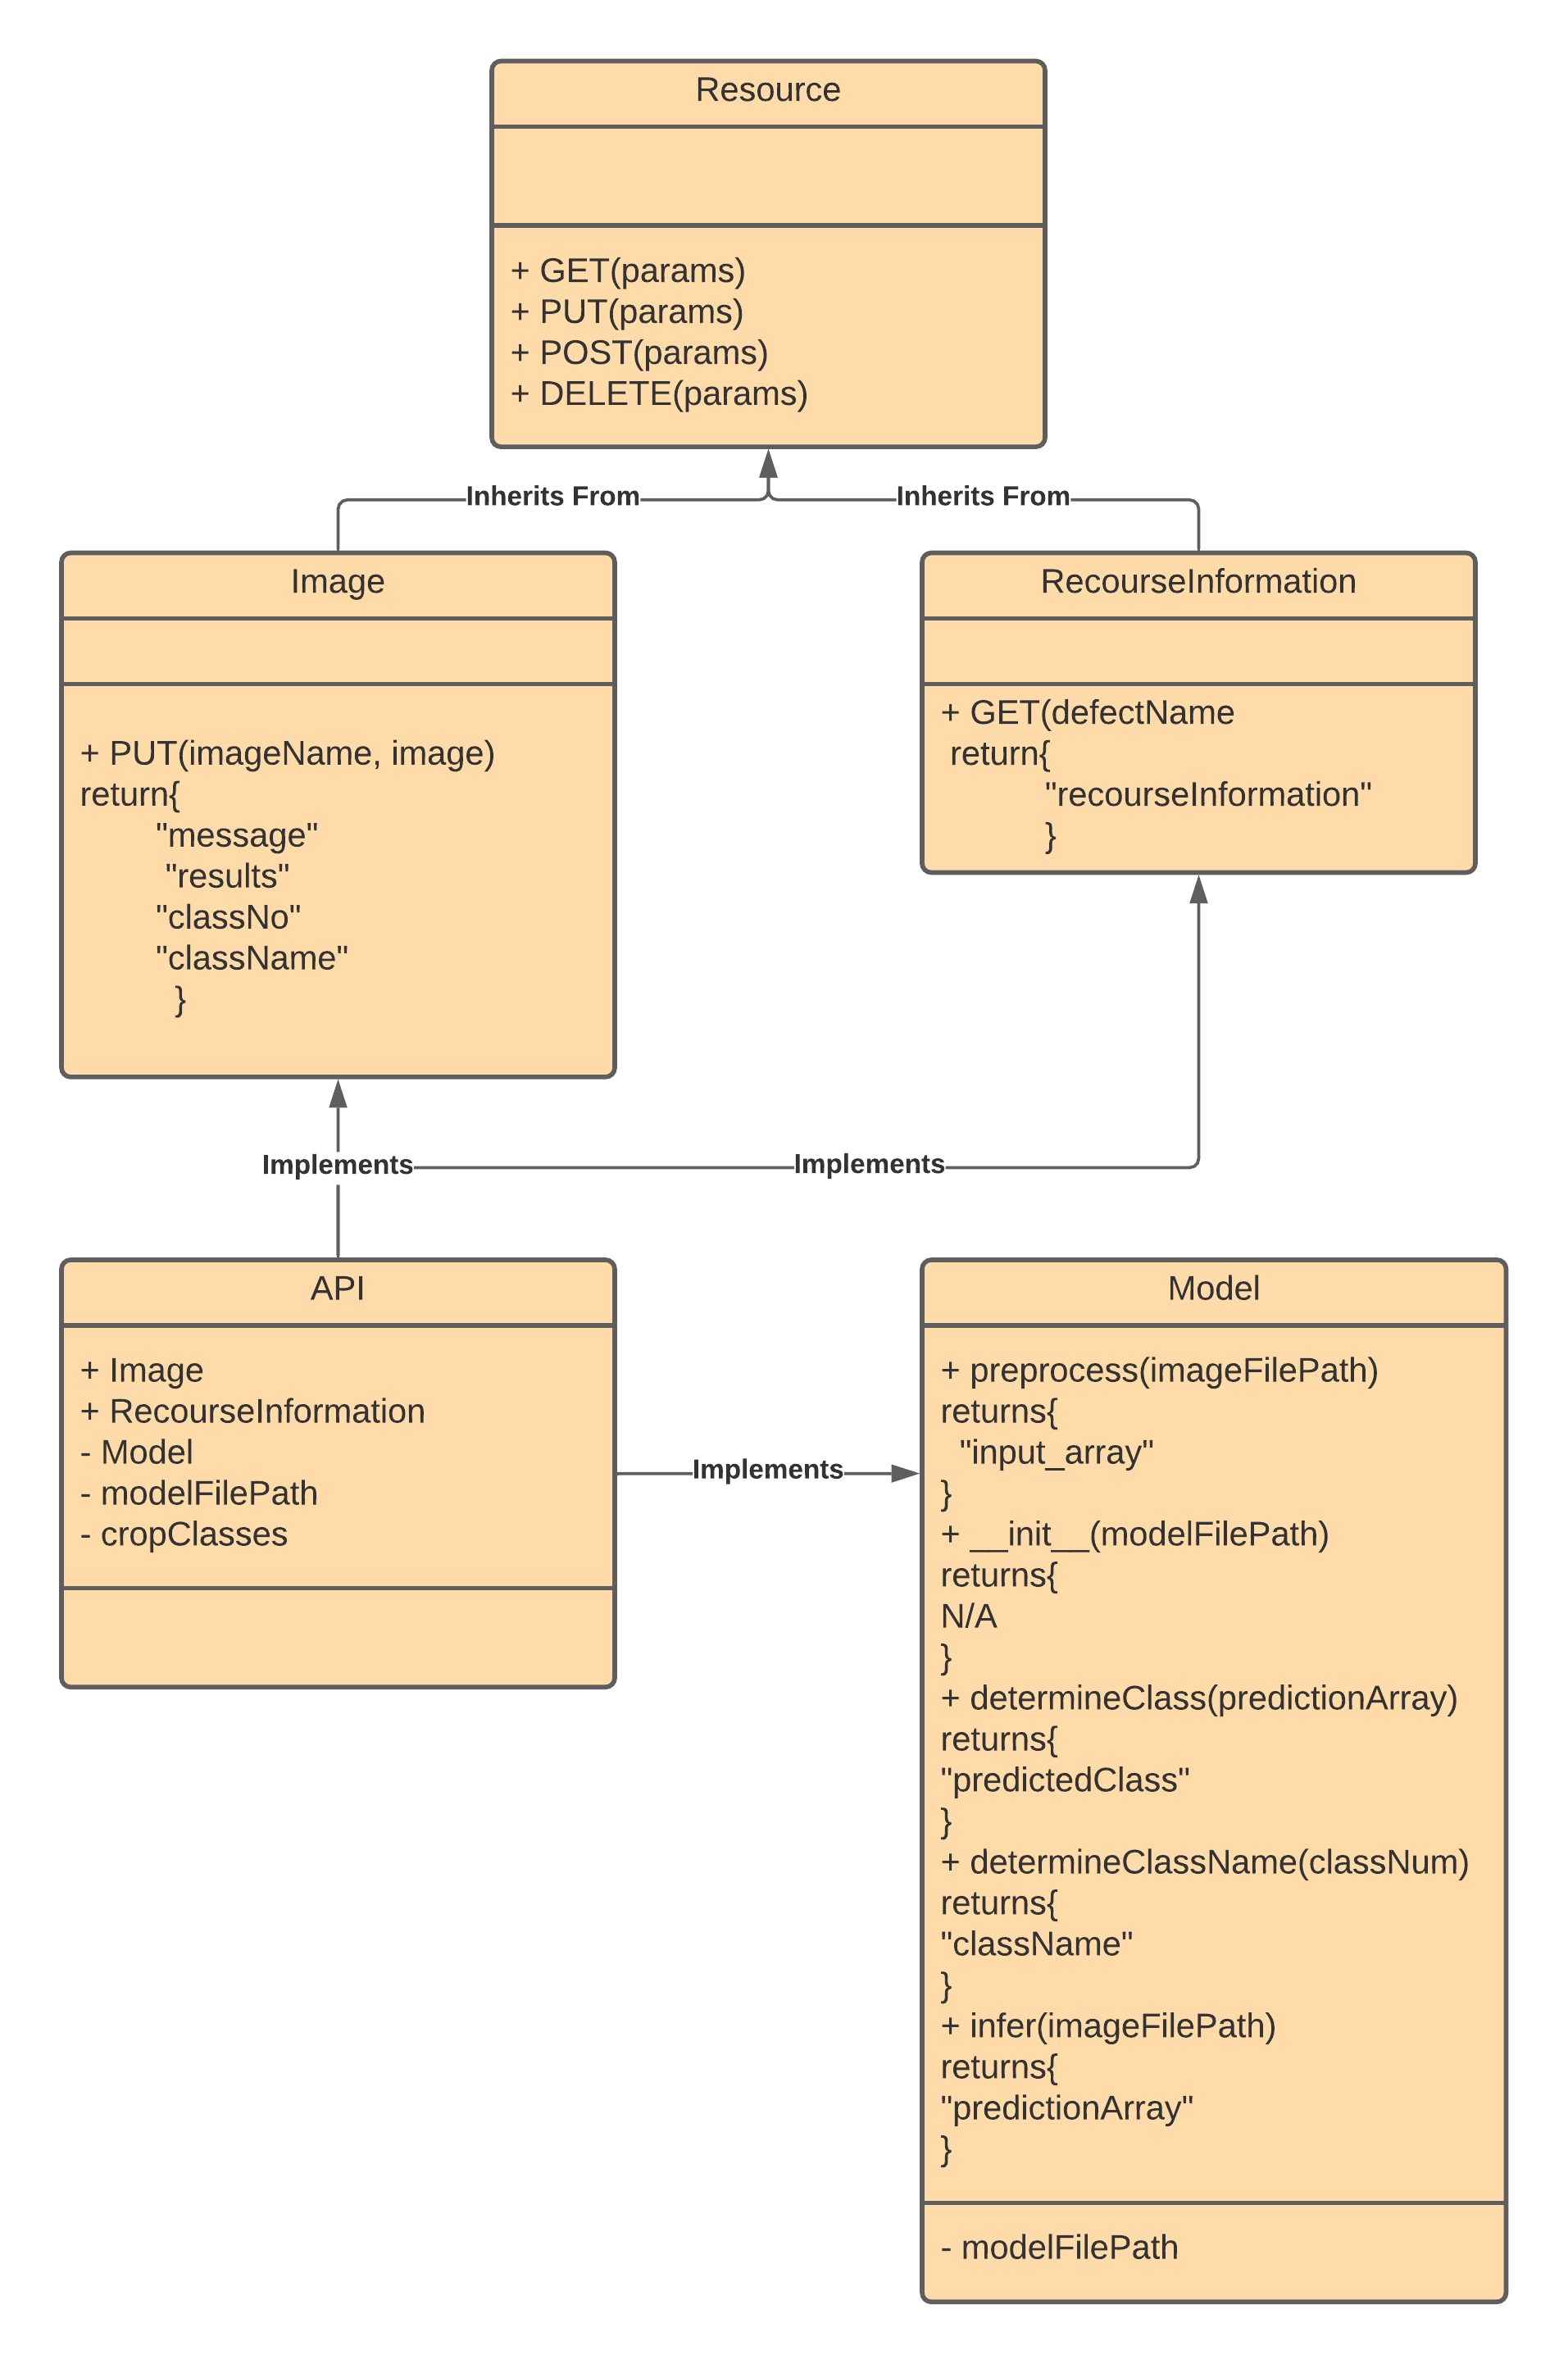
\includegraphics[scale=0.7]{Images/API_InheritenceV3}
        \caption{Backend Class Diagram}
        \label{fig:api_inheritence}
      \end{center}
    \end{figure}

    \subsubsection{Front-End}
      Using the Vue.js webpack framework means the front-end will be split in to components. A component acting much like an endpoint in an API. Each component will have it's own set of functions and data, with the purpose of seprerating functionality of the UI in to manageable subsets of functionality and styling with the objective being to decouple dependancies between compoonents as much as possible. This helps simplify the development process as it seperates the problem in to distinct parts and it helps with maintinence, allowing them to be tested and developed on in isolation.
      \par
      UI components will be defined using Hypertext Markup language (HTML) and Cascading Style Sheets (CSS). Interativity will be scripted in Javascript. All three extremely common in web development. %With some of the earliest pages of the world wide web in 1990 being defined in HTML1.0 now developed to HTML4.0 (citep html4.0 spec).
      \par
      The main functionality of the web-app will be uploading an image to be analysed by the CNN and recieving a prediciton of which defect is/isn't present. This will be conducted by a single component. Once a prediction has been made, the user can choose to see more information (consisting of images and recourse information) about the defect, which will be handled by two further components.
      \par
      Responses from the API will come in JSON format. JSON is a structured data language and stores data heirachically. This leads to dictonaries and lists of arbitrary depth in a tree structure. Much the same as XML or a filesystem. JSON is a very common language when dealing with webservices and is considered the norm to be the response of an API.
      \par
      The application is made with the intention that as much data processing, such as determining which class is predicted, image preprocessing and determining of defect image URL's, defect names etc. is handled on the back-end, meaning that any client wishing to interact with the API does not have to implement these features themselves. Therefore, all functionality implemented in the web app will concern the consumption of user input and display of API response.
      \par
      This means the navigation drop-downs, defect images and recourse/prevention information are all served dynamically through the API and can be scaled more easily than if the information was stored on the frontend. Because the content is dynamic, any client consuming the information won't have to manually update their defect list or defect names if the CNN model changes. This is in-line with the don't repeat yourself (DRY) principle. Having two places where what is supposed to be the same information is stored is an immediate 'code smell' and can easily lead to bugs. This also stands true for methods which enact some kind of bisuness logic. For instance it would not be best practice to implement the algorithm which re-scales the image both on the front and back end, as the size the algorithm needs to re-scale to may change, or a better method for re-scaling the image may become apparent, this would cascade to changing two parts of the system.
      % This stands true for any function that is supposed to enact some kind of bisuness logic. For instance the government may have a policy as to which kind of string is a valid national insurance number (NIN). This could then lead to multiple implementations of a NIN checker, being written for multiple applications accross the governments software suite, one in javascript for a driving licence sign up web application, one in python for an internal police database management system etc. And all become defunkt if this peice of 'bisuness logic' changes. Therefore, this calls for the software to by written dynamically from metadata. And requries the creation of a higher level language compiler, to compile metadata into a different high level language such as Java, C++, Python etc. Or at least get the programmer most of the way to the solution by defining necessary method names and declarations along with return types, error values etc.

    \subsection{Hosting}
      To make the application accessible on the internet one will utilize virtual machines (VM's) running linux, hosted in the cloud. There will be three VM's, one to host the front-end, back-end and the other to host the defect images. In all cases nginx will be used to create HTTP servers that will handle all functionality regarding the HTTP protocol and the socket layer.
      \par
      Aside from creating backups of work, version control allows production environments (in this case the VM's) to be easily updated with new features, simply by pulling the latest changes from the repo, installing any new dependencies and re-building the application.

      \subsection{Choosing The CNN Architecture}
      The initial architecture one experimented with was the InceptionNetV3, the reason being that one already had a familiarity with the architecture and therefore could rationalise about what may need to change in order to get better performance on the target dataset if initial experiments were not satisfactory. One opted to use a model pre-trained on the ILSSVRC dataset and fine-tune it to suit the crop dataset. This resulted in the model taking around six hours to train over an epoch (using Google Colab GPU runtime) and also drastically overtiffing the training data. One reasoned that the vast number of weights could be to blame for both problems, firstly the more weights the greater the training time, secondly, more filters leads to the network making less generalisations and being able to store many bespoke feature maps to target subsets or perhaps even individual images. Hence when it comes to an unseen example it's feature maps are not generic enough to aid in identifying the unseen image. Therefore one decided to use a a smaller network, 'EfficentNetB0', a network available as a pre-trained\footnote{on the ILSSVRC dataset}[1] CNN through the Keras library. For comparison  the InceptionV3 architecture is 92mb and contains 23,851,784 parameters (weights) whereas the EfficientNetB1 is 29mb and contains 5,330,571 parameters (approx 1/3 the parameters). Fine-tuning this network proved very successfull, acheiving a 98.6\% accuracy. For this dataset, due to the fact all classes the network is classifiying for are relatively similar, less feature maps are needed to generalise about the forms present. To contrast, a network that must classify 100 different classes ranging from a baseball to a shark. with all objects present in different contexts, for instance a closeup of the baseball sat on a table, and a long range shot of it mid flight across the stadium. And it becomes easy to see why so many filters would be necessary. If we take the crop-example we see all images are closeups of leaves with a neutral background. Therefore it is possible to generalise about this smaller subset of possible images with fewer filters. In fact few parameters becomes a desirable quality of the network as it forces the network to generalise as it does not have the ability to 'memorise' all the individual training images.


      %designing the system to include a relational database such MySql, as one beleives there may be a need to handle a large amount of  relational data. Later in the project, one realizes they only need the application to be able to retrieve dispirate and simple data, so one drops the database, in favour of using the hierachical storage of the filesystem and structured data languages such as JSON or XML. Another example being,
      % Such as, adding more libraries to the project will have the knock on effect of increasing the amount of time spent    are one of many factors that feed-into one another such as usability, speed of excecution and speed of creation feed in to one-another.

    \subsubsection{CNN Data and Training}
      One of the most important parts when creating a CNN is the data it is trained on \citep{Halevy2009}. The more properly labled data the network sees, the better. The most comprehensive dataset available (and the one which will mostly be used) is the Plant Village dataset. it contains 54303 images of healthy and unhealthy leaf images, in 38 categories divided by species and disease. This dataset also contains pre-segmented\footnote{meaning the background has been blacked out}[1] versions of all the images. This dataset was used in two seperate studies cited in the literature review.
      \par
      Other datasets that may be used to pre-train the network before are the CIFAR10, CIFAR100 \& ILSVRC datasets. These datasets are not specifically plant based, but may benefit the network to build initial feature maps. In \citep{Choi} the authors used networks pre-trained on generic data such as the datasets mentioned.
      \par
      One unfortunate aspect was the fact that one was unable to obtain a dataset that reflected plant defects other than diseases, such as nitrogen/water/heat deficiencies.


\subsection{Technologies \& Libraries}
  \subsubsection{Vue.js}
    Vue.js allows for rapid creation of usable websites thanks to its webpack framework, which handles most of the boilerplate needed to handle URL routing and overall structure. It is also considered easy to learn when compared to React and Angular \citep{StudiengangBachelor} which for this project is optimal. Although Vue is currently less popular than React and Angular its popularity is rising, which means its not entirely redundant to learn from an employability standpoint. Vue is a component based framework, meaning that it creates a structure to allow the programmer to utilize component technologies to build the website. The component technologies are; custom elements, which allow the programmer to embed javascript code in to either existing HTML elemnts by inheriting from them, or creating entirely new ones. HTML templates, which allows for sections of HTML to be re-used throuought the application, for instance navigation bars. Also, Shadow DOM's, which allow for DOM elements to contain sub-trees of elements, this is to aid in encapsulating the scope of the contained scripting and styling, meaning individual elements can have their own layers of encapsulation.
  \subsubsection{Bootstrap}
    Bootstrap is a CSS framework that has predefined classes for styling HTML elements, this helps with the asthetics of the webpage. For a solo developer this can allow for more time to spent on making the functionality more robust and cut down time spent on appearance.
  \subsubsection{Jupyter Notebook / Google Colab}
    The Jupyter Python environment allows for easy prototyping of code, it allows the programmer to write code in cells that can be run independently and not necessarily in the same order each time. In the case of Colab, it allows for the usage of google servers and Graphics Processing Units (GPUS) which can be used to train neural networks. With the benefit of being able to then save the trained weights for usage elsewhere.
  \subsubsection{Tensorflow \& Keras}
    These Python libraries allow for the creation of complex CNN architectures by abstracting away the underlying matrix/tensor multiplication of deep learning. This allows the programmer to declare relationships between CNN features such as convolutional layers, batch normalisation, dropout etc. Without having to construct their inner workings, it also allows for the creation of user defined layers, so adding in ones own bespoke functionality for a layer of the CNN is possible. These libraries are ubiquitous in the machine vision sector, with cutting edge models being created
  \subsubsection{Nginx}
    NginX is a web server. This software, installed on the virtual machines (VM's) hosting, front/back end and files. Handles incoming HTTP protocol requests on ports it is configured to listen to, and serves content accordingly. Additionally, if the need arises, NginX can be used as a load balancer. Taking incoming requests and distributing them amongst the back-end servers via a reverse-proxy. With the reverse-proxy aproach it is also possible to cache response data. Reducing load on the back-end. It can also be used to create IP address white/black lists, set file upload limits, keep access logs and more.
  \subsubsection{Gunicorn}
    Gunicorn is another technology used to host the application. This time it is used to interface with the Flask API. It is a Web Server Gateway Interface (WSGI) HTTP server. This gives an interface to the API to allow it to send data back and forth between the web server, NginX.
  \subsubsection{Flask/FLask-Restful}
    These libraries provide a framework for creating RESTFul API's in Python and gives the Resource class to inherit from for each endpoint. Flask also provides a built in development server for testing the appliation on your local machine.
  \subsubsection{Numpy}
    This Python library is essential when performing mathematical operations with Python, especially matrix multiplication, as in this case it is over 10,000 times faster than vanilla python. Other mathematical operations are also often orders of magnitude faster than vanilla. Aditionally it adds the ability to use 'proper' arrays and not lists which are extensible, this means less memory is needed.\citep{mediumAnuradaNumpy}
  \subsubsection{Node \& Node Package Manager}
    Node creates an environment for JavaScript to be run outside of the browser environment. This is especially useful during development as it allows the developer to create a local Node server to test the code. Node's package manager checks for any dependencies the code may have and automatically installs apropriate versions, ensuring that the project does not have incompatible versions of dependencies installed simultaneously. As this can easily be a source of frustration when trying to handle multiple dependencies. This also means that whenever a new dependency is added in development, the package manager will automatically add install it in production during the build process.

\section{Requirements}
For assessing requirement priority one will employ the MOSCOW method \citep{Clegg199410.5555/561543}. This creates subcategory of requirments with the headings Must/Should/Could/Won't - have. The contents of the categories can change during development in light of development progress. Items placed in the Won't-have category prevent the process of 'scope-creep'.
\begin{enumerate}
  \item Must Have
  \begin{enumerate}
    \item CNN that is capable of classifying at least 2 different defects across 2 different plant species.
    \item An API that allows communication from the UI to the CNN
    \item API must be able to receive images.
      \begin{itemize}
        \item Accepted formats being .jpg \& .png
      \end{itemize}
    \item API must return defect information, which will be an array of probability values for each defect class
    \item API must return recourse information.
    \item Application must display images that show the predicted defect.
      \begin{itemize}
        \item These images may be stored either on a seperate server to the front-end. Perhaps in the API servers 'static folder'. Alternatively they will be bundled with the front end.
      \end{itemize}
  	\item The API will be robust enough to handle the receipt of erroneous requests.
  	\item A python backend that will handle image classification using a CNN.
  	\item A UI that will allow the user to upload an image to be analysed.
    \begin{itemize}
      \item The user will be able to choose an image file from their local storage using a file explorer popup.
    \end{itemize}
  	\item The UI will display information regarding the likelihood of each kind of possible defect.
  	\item To display the relevant images that fit the description of the most likely defects.
  	\item To display recourse information to rectify the defect.
  	\item Collecting, cleaning and pre-processing the image data.
    \item Artificially grow the dataset by performing translations/rotations/adding noise to the images to make the training data more comprehensive.
  \end{enumerate}
  \item Should Have
  \begin{enumerate}
    \item A page to allow users to see a gallery of images sorted by
      defect type.
    \item The CNN should be able to classify at least 7 different defects across at least two different plant species.
    \item The CNN should acheive at least 80\% accuracy at classifying all different classes of defect in a held out test set that contains an equal number of each class.
  	\item Regularisation techniques to prvent the NN overfitting.
  \end{enumerate}
  \item Could Have
  \begin{enumerate}
      \item Mobile device support.
    \item Ability for users to add additional information about the crop
      to determine the defect.
  \end{enumerate}
  \item Won't Have
\end{enumerate}
% \section{Testing and Implementation details}


% \section{Justification of Implementation Choices}
